% Options for packages loaded elsewhere
\PassOptionsToPackage{unicode}{hyperref}
\PassOptionsToPackage{hyphens}{url}
%
\documentclass[
]{book}
\usepackage{lmodern}
\usepackage{amssymb,amsmath}
\usepackage{ifxetex,ifluatex}
\ifnum 0\ifxetex 1\fi\ifluatex 1\fi=0 % if pdftex
  \usepackage[T1]{fontenc}
  \usepackage[utf8]{inputenc}
  \usepackage{textcomp} % provide euro and other symbols
\else % if luatex or xetex
  \usepackage{unicode-math}
  \defaultfontfeatures{Scale=MatchLowercase}
  \defaultfontfeatures[\rmfamily]{Ligatures=TeX,Scale=1}
\fi
% Use upquote if available, for straight quotes in verbatim environments
\IfFileExists{upquote.sty}{\usepackage{upquote}}{}
\IfFileExists{microtype.sty}{% use microtype if available
  \usepackage[]{microtype}
  \UseMicrotypeSet[protrusion]{basicmath} % disable protrusion for tt fonts
}{}
\makeatletter
\@ifundefined{KOMAClassName}{% if non-KOMA class
  \IfFileExists{parskip.sty}{%
    \usepackage{parskip}
  }{% else
    \setlength{\parindent}{0pt}
    \setlength{\parskip}{6pt plus 2pt minus 1pt}}
}{% if KOMA class
  \KOMAoptions{parskip=half}}
\makeatother
\usepackage{xcolor}
\IfFileExists{xurl.sty}{\usepackage{xurl}}{} % add URL line breaks if available
\IfFileExists{bookmark.sty}{\usepackage{bookmark}}{\usepackage{hyperref}}
\hypersetup{
  pdftitle={exposomeShiny User's Guide},
  pdfauthor={Escribà Montagut, Xavier; González, Juan R.},
  hidelinks,
  pdfcreator={LaTeX via pandoc}}
\urlstyle{same} % disable monospaced font for URLs
\usepackage{color}
\usepackage{fancyvrb}
\newcommand{\VerbBar}{|}
\newcommand{\VERB}{\Verb[commandchars=\\\{\}]}
\DefineVerbatimEnvironment{Highlighting}{Verbatim}{commandchars=\\\{\}}
% Add ',fontsize=\small' for more characters per line
\usepackage{framed}
\definecolor{shadecolor}{RGB}{248,248,248}
\newenvironment{Shaded}{\begin{snugshade}}{\end{snugshade}}
\newcommand{\AlertTok}[1]{\textcolor[rgb]{0.94,0.16,0.16}{#1}}
\newcommand{\AnnotationTok}[1]{\textcolor[rgb]{0.56,0.35,0.01}{\textbf{\textit{#1}}}}
\newcommand{\AttributeTok}[1]{\textcolor[rgb]{0.77,0.63,0.00}{#1}}
\newcommand{\BaseNTok}[1]{\textcolor[rgb]{0.00,0.00,0.81}{#1}}
\newcommand{\BuiltInTok}[1]{#1}
\newcommand{\CharTok}[1]{\textcolor[rgb]{0.31,0.60,0.02}{#1}}
\newcommand{\CommentTok}[1]{\textcolor[rgb]{0.56,0.35,0.01}{\textit{#1}}}
\newcommand{\CommentVarTok}[1]{\textcolor[rgb]{0.56,0.35,0.01}{\textbf{\textit{#1}}}}
\newcommand{\ConstantTok}[1]{\textcolor[rgb]{0.00,0.00,0.00}{#1}}
\newcommand{\ControlFlowTok}[1]{\textcolor[rgb]{0.13,0.29,0.53}{\textbf{#1}}}
\newcommand{\DataTypeTok}[1]{\textcolor[rgb]{0.13,0.29,0.53}{#1}}
\newcommand{\DecValTok}[1]{\textcolor[rgb]{0.00,0.00,0.81}{#1}}
\newcommand{\DocumentationTok}[1]{\textcolor[rgb]{0.56,0.35,0.01}{\textbf{\textit{#1}}}}
\newcommand{\ErrorTok}[1]{\textcolor[rgb]{0.64,0.00,0.00}{\textbf{#1}}}
\newcommand{\ExtensionTok}[1]{#1}
\newcommand{\FloatTok}[1]{\textcolor[rgb]{0.00,0.00,0.81}{#1}}
\newcommand{\FunctionTok}[1]{\textcolor[rgb]{0.00,0.00,0.00}{#1}}
\newcommand{\ImportTok}[1]{#1}
\newcommand{\InformationTok}[1]{\textcolor[rgb]{0.56,0.35,0.01}{\textbf{\textit{#1}}}}
\newcommand{\KeywordTok}[1]{\textcolor[rgb]{0.13,0.29,0.53}{\textbf{#1}}}
\newcommand{\NormalTok}[1]{#1}
\newcommand{\OperatorTok}[1]{\textcolor[rgb]{0.81,0.36,0.00}{\textbf{#1}}}
\newcommand{\OtherTok}[1]{\textcolor[rgb]{0.56,0.35,0.01}{#1}}
\newcommand{\PreprocessorTok}[1]{\textcolor[rgb]{0.56,0.35,0.01}{\textit{#1}}}
\newcommand{\RegionMarkerTok}[1]{#1}
\newcommand{\SpecialCharTok}[1]{\textcolor[rgb]{0.00,0.00,0.00}{#1}}
\newcommand{\SpecialStringTok}[1]{\textcolor[rgb]{0.31,0.60,0.02}{#1}}
\newcommand{\StringTok}[1]{\textcolor[rgb]{0.31,0.60,0.02}{#1}}
\newcommand{\VariableTok}[1]{\textcolor[rgb]{0.00,0.00,0.00}{#1}}
\newcommand{\VerbatimStringTok}[1]{\textcolor[rgb]{0.31,0.60,0.02}{#1}}
\newcommand{\WarningTok}[1]{\textcolor[rgb]{0.56,0.35,0.01}{\textbf{\textit{#1}}}}
\usepackage{longtable,booktabs}
% Correct order of tables after \paragraph or \subparagraph
\usepackage{etoolbox}
\makeatletter
\patchcmd\longtable{\par}{\if@noskipsec\mbox{}\fi\par}{}{}
\makeatother
% Allow footnotes in longtable head/foot
\IfFileExists{footnotehyper.sty}{\usepackage{footnotehyper}}{\usepackage{footnote}}
\makesavenoteenv{longtable}
\usepackage{graphicx,grffile}
\makeatletter
\def\maxwidth{\ifdim\Gin@nat@width>\linewidth\linewidth\else\Gin@nat@width\fi}
\def\maxheight{\ifdim\Gin@nat@height>\textheight\textheight\else\Gin@nat@height\fi}
\makeatother
% Scale images if necessary, so that they will not overflow the page
% margins by default, and it is still possible to overwrite the defaults
% using explicit options in \includegraphics[width, height, ...]{}
\setkeys{Gin}{width=\maxwidth,height=\maxheight,keepaspectratio}
% Set default figure placement to htbp
\makeatletter
\def\fps@figure{htbp}
\makeatother
\setlength{\emergencystretch}{3em} % prevent overfull lines
\providecommand{\tightlist}{%
  \setlength{\itemsep}{0pt}\setlength{\parskip}{0pt}}
\setcounter{secnumdepth}{5}
\usepackage{booktabs}
\usepackage[]{natbib}
\bibliographystyle{apalike}

\title{exposomeShiny User's Guide}
\author{Escribà Montagut, Xavier; González, Juan R.}
\date{2020-10-13}

\begin{document}
\maketitle

{
\setcounter{tocdepth}{1}
\tableofcontents
}
\hypertarget{overview}{%
\chapter{Overview}\label{overview}}


\includegraphics[width=0.5\textwidth,height=\textheight]{images/athlete.png}

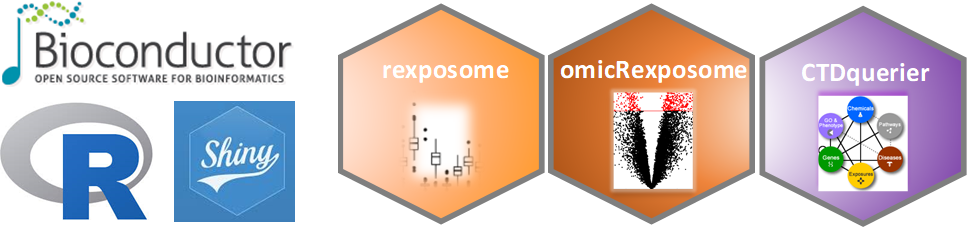
\includegraphics[width=0.6\textwidth,height=\textheight]{images/logo.png}

exposomeShiny is a data analysis toolbox with the following features:

\begin{itemize}
\tightlist
\item
  Data handling: imputation, LOD, transformation, \ldots{}
\item
  Exposome characterization
\item
  Exposome-wide association analysis
\item
  Multivariate association
\item
  Omic data integration
\item
  Post-omic data analysis: CTD database
\end{itemize}

To do so, exposomeShiny relies on previously existent Bioconductor packages (rexposome, omicRexposome and CTDquerier), it uses them in a seamless way so the final user of exposomShiny can perform the same studies that would conduct using the Bioconductor packages but without writing a single line of code.

\hypertarget{setup}{%
\chapter{Setup}\label{setup}}

There are two different ways of seting up and using exposomeShiny

\hypertarget{downloading-the-source-files-installing-the-libraries-and-running-the-application}{%
\section{Downloading the source files, installing the libraries and running the application}\label{downloading-the-source-files-installing-the-libraries-and-running-the-application}}

The user can choose to download the source code of the shiny application and install all the required libraries on their local R installation. Make sure \href{https://cran.r-project.org/bin/windows/Rtools/history.html}{Rtools} is installed to use this method.

\begin{Shaded}
\begin{Highlighting}[]
  \CommentTok{# Set working directory}
\KeywordTok{setwd}\NormalTok{(}\DataTypeTok{dir =} \StringTok{"/some/path/"}\NormalTok{)}
      
  \CommentTok{# Download zip}
\KeywordTok{download.file}\NormalTok{(}\DataTypeTok{url =} \StringTok{"https://github.com/isglobal-brge/exposomeShiny/archive/master.zip"}\NormalTok{, }\DataTypeTok{destfile =} \StringTok{"master.zip"}\NormalTok{)}

  \CommentTok{# Unzip the .zip to the working directory}
\KeywordTok{unzip}\NormalTok{(}\DataTypeTok{zipfile =} \StringTok{"master.zip"}\NormalTok{)}

  \CommentTok{# Set the working directory inside the downloaded folder}
\KeywordTok{setwd}\NormalTok{(}\DataTypeTok{dir =} \StringTok{"/some/path/exposomeShiny-master"}\NormalTok{)}
\end{Highlighting}
\end{Shaded}

Now all the source files are downloaded to the location of chose and the working directory moved to the correct folder, to start the project, open the \texttt{Rproj} file by clicking it on the Files explorer of RStudio.

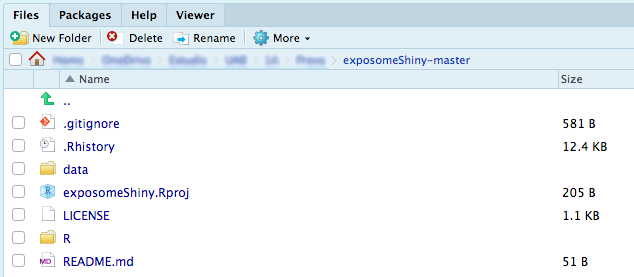
\includegraphics{images/setup1.png}

Once the project is loaded, the file found on the source folder called \texttt{installer.R} has to be sourced and run. This will install the newest versions of the packages required by Exposome Shiny on this R session. To do so, run the following code on the RStudio console.

\begin{Shaded}
\begin{Highlighting}[]
\KeywordTok{source}\NormalTok{(}\StringTok{"installer.R"}\NormalTok{)}
\end{Highlighting}
\end{Shaded}

This is only needed on the first run, once completed it doesn't need to be done prior to launching the application itself any other time.

Now everything is ready to launch the Shiny application. To do so there a two approaches, one is to open the \texttt{ui.R} or the \texttt{server.R} files that are inside the \texttt{R} folder and press \texttt{Run\ App}.

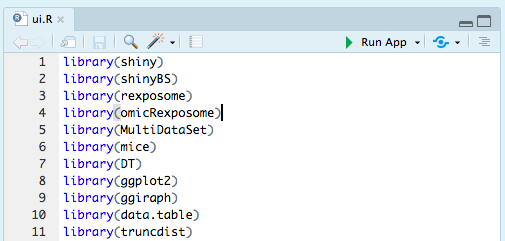
\includegraphics{images/setup2.png}

Or the other option is to input the following command on the console.

\begin{Shaded}
\begin{Highlighting}[]
\NormalTok{shiny}\OperatorTok{::}\KeywordTok{runApp}\NormalTok{(}\StringTok{'R'}\NormalTok{)}
\end{Highlighting}
\end{Shaded}

\hypertarget{pulling-the-official-docker-image-from-dockerhub}{%
\section{Pulling the official Docker image from DockerHub}\label{pulling-the-official-docker-image-from-dockerhub}}

If there's any troubble downloading the required R packages to make exposomeShiny work, there's the option of using Docker. It has the disadvantage of being a little bit difficult to install on a Windows machine, however, it's extremely simple on a Mac OS X / Linux environment. For the Windows users refer to the following links for instructions on how to install Docker and setup you machine to run WSL2 and launch bash commands on Windows \href{https://docs.docker.com/docker-for-windows/install-windows-home/}{1}, \href{https://blog.nillsf.com/index.php/2020/02/17/setting-up-wsl2-windows-terminal-and-oh-my-zsh/}{2}, \href{https://docs.docker.com/docker-for-windows/wsl/}{3}.

To download and launch exposomeShiny, execute the following command on a bash terminal(make sure Docker is running, if not search for the \texttt{Docker\ Desktop} app and launch it).

\begin{Shaded}
\begin{Highlighting}[]
\ExtensionTok{docker}\NormalTok{ run --rm -p 80:80 brgelab/exposome-shiny}
\end{Highlighting}
\end{Shaded}

This command will download the Docker image of exposomeShiny (be aware it weights \textasciitilde{} 3 GB, so if your internet connection is slow it may take a while) and run a container with it. The container will be exposed on the local port 80 and it will render on that port the application itself, so to start using exposomeShiny open your web browser and go to the site

\begin{Shaded}
\begin{Highlighting}[]
\ExtensionTok{localhost}\NormalTok{:80}
\end{Highlighting}
\end{Shaded}

At the beginning it may take some time for the application to render, this is because all the needed R libraries are being loaded, to be sure the container is actually working, take a look at the terminal where you inputed the Docker command, there you will see all the R verbose stating the libraries are being loaded.

Once the user has finished using exposomeShiny, the container needs to be stopped to avoid wasting CPU resources, to do so, input the following command on a bash terminal (the command needs to be inputed on a new bash window):

\begin{Shaded}
\begin{Highlighting}[]
\ExtensionTok{docker}\NormalTok{ container ls}
\end{Highlighting}
\end{Shaded}

This will prompt all the running containers, find the one with the NAMES \texttt{brgelab/exposome-shiny} and copy it's CONTAINER ID, then input the following bash command:

\begin{Shaded}
\begin{Highlighting}[]
\ExtensionTok{docker}\NormalTok{ stop xxxxxxxxxxxx}
\end{Highlighting}
\end{Shaded}

Where xxxxxxxxxxxx is the CONTAINER ID.

To run the application again, just enter the first bash command (\texttt{docker\ run\ -\/-rm\ -p\ 80:80\ brgelab/exposome-shiny}), since it has already been downloaded, the application is cached on the computer and it will launch straight away. If the user wants to remove the Docker image from the computer, input the following bash command:

\begin{Shaded}
\begin{Highlighting}[]
\ExtensionTok{docker}\NormalTok{ image rm brgelab/exposome-shiny}
\end{Highlighting}
\end{Shaded}

\hypertarget{data-sets}{%
\chapter{Data sets}\label{data-sets}}

\hypertarget{exposome-dataset}{%
\section{Exposome dataset}\label{exposome-dataset}}

The exposome is composed of three different files (in \texttt{*.csv} format). Those files are refered inside the Shiny as exposures, description and phenotypes. Their content is the following:

\begin{itemize}
\tightlist
\item
  The \texttt{exposures} file contains the measures of each exposure for all the individuals included on the analysis. It is a matrix-like file having a row per individual and a column per exposures. It must includes a column with the subject's identifier.
\item
  The \texttt{description} file contains a row for each exposure and, at last, defined the families of exposures. Usually, this file incorporates a description of the exposures, the matrix where it was obtained and the units of measurement among others.
\item
  The \texttt{phenotypes} file contains the covariates to be included in the analysis as well as the health outcomes of interest. It contains a row per individual included in the analysis and a column for each covariate and outcome. Moreover, it must include a column with the individual's identifier.
\end{itemize}

A visual representation of the three matrices and how they correlate is the following.

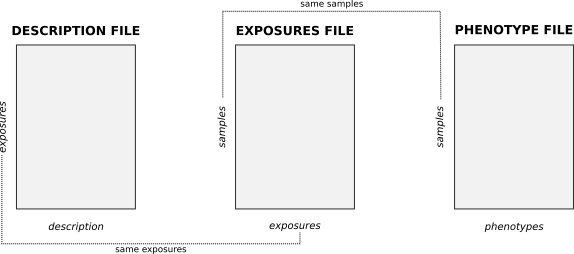
\includegraphics{images/exposome_dataset_struct.png}

Exposures data file example:

\begin{verbatim}
id    bde100  bde138  bde209  PFOA    ...
sub01  2.4665  0.7702  1.6866  2.0075 ...
sub02  0.7799  1.4147  1.2907  1.0153 ...  
sub03 -1.6583 -0.9851 -0.8902 -0.0806 ... 
sub04 -1.0812 -0.6639 -0.2988 -0.4268 ... 
sub05 -0.2842 -0.1518 -1.5291 -0.7365 ... 
...   ...     ...     ...     ...
\end{verbatim}

Description data file example:

\begin{verbatim}
exposure  family  matrix         description
bde100    PBDEs   colostrum       BDE 100 - log10
bde138    PBDEs   colostrum       BDE 138 - log10
bde209    PBDEs   colostrum       BDE 209 - log10
PFOA      PFAS    cord blood      PFOA - log10
PFNA      PFAS    cord blood      PFNA - log10
PFOA      PFAS    maternal serum  PFOA - log10
PFNA      PFAS    maternal serum  PFNA - log10
hg        Metals  cord blood      hg - log 10
Co        Metals  urine           Co (creatinine) - log10
Zn        Metals  urine           Zn (creatinine) - log10
Pb        Metals  urine           Pb (creatinine) - log10
THM       Water   ---             Average total THM uptake - log10
CHCL3     Water   ---             Average Chloroform uptake - log10
BROM      Water   ---             Average Brominated THM uptake - log10
NO2       Air     ---             NO2 levels whole pregnancy- log10
Ben       Air     ---             Benzene levels whole pregnancy- log10
\end{verbatim}

Phenotypes data file example:

\begin{verbatim}
id    asthma   BMI      sex  age  ...
sub01 control  23.2539  boy  4    ...
sub02 asthma   24.4498  girl 5    ...
sub03 asthma   15.2356  boy  4    ...
sub04 control  25.1387  girl 4    ...
sub05 control  22.0477  boy  5    ...
...   ...      ...      ...  ...
\end{verbatim}

\hypertarget{omics-dataset}{%
\section{Omics dataset}\label{omics-dataset}}

The omics data inputed to the Shiny must be provided as an \texttt{*.RData}. This file has to contain an ExpressionSet, which is an S4 object. This object is a data container of the Bioconductor toolset.

For further information on ExpressionSet and how to create and manipulate them, please visit the \href{https://www.bioconductor.org/packages/devel/bioc/vignettes/Biobase/inst/doc/ExpressionSetIntroduction.pdf}{official documentation} and this \href{https://kasperdanielhansen.github.io/genbioconductor/html/ExpressionSet.html}{selected vignette}.

\hypertarget{bioconductor-packages}{%
\chapter{Bioconductor packages}\label{bioconductor-packages}}

This Shiny application is a front end support for other Bioconductor packages in order to provide a comfortable environment on to conduct different analysis with those packages. In concrete the packages are \href{https://www.bioconductor.org/packages/release/bioc/html/rexposome.html}{rexposome}, \href{https://bioconductor.org/packages/release/bioc/html/omicRexposome.html}{omicRexposome} and \href{http://www.bioconductor.org/packages/release/bioc/html/CTDquerier.html}{CTDquerier}.

\hypertarget{rexposome}{%
\section{rexposome}\label{rexposome}}

Rexposome is a package that allows to explore the exposome and to perform association analyses between exposures and health outcomes.

\hypertarget{omicrexposome}{%
\section{omicRexposome}\label{omicrexposome}}

OmicRexposome is a package that systematizes the association evaluation between exposures and omic data, taking advantage of MultiDataSet for coordinated data management, rexposome for exposome data definition and limma for association testing. Also to perform data integration mixing exposome and omic data using multi co-inherent analysis (omicade4) and multi-canonical correlation analysis (PMA).

\hypertarget{ctdquerier}{%
\section{CTDquerier}\label{ctdquerier}}

CTDquerier is a package to retrieve and visualize data from the \href{http://ctdbase.org/}{Comparative Toxicogenomics Database}. The downloaded data is formated as DataFrames for further downstream analyses.

\hypertarget{analysis-flowcharts}{%
\chapter{Analysis flowcharts}\label{analysis-flowcharts}}

\hypertarget{exposome-analysis}{%
\section{Exposome analysis}\label{exposome-analysis}}

As any user would need to do using the Bioconductor packages (rexposome, omicRexposome and CTDquerier) when performing an analysis using an \texttt{R} script, there is some kind of flow (or pipeline) to follow in order to get to the results, this is also true on rexposomeShiny, even though it's a seamless and codeless integration of the packages there's still some need for a flowchart to get the desired results. All the required flowcharts will be detailed with a box flowchart as well as screenshots of exposomeShiny in order to provide extra guidance if needed.

\hypertarget{lod-imputation}{%
\subsection{LOD imputation}\label{lod-imputation}}

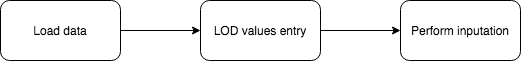
\includegraphics{images/analysis1_1.png}

Input the exposures, description and phenotypes files and load them into the application. On the right of the file browsers, there are four text fields to input the following:

\begin{itemize}
\tightlist
\item
  Column name in the \emph{description} file that contains the exposures
\item
  Column name in the \emph{description} file that contains the families\\
\item
  Column name in the \emph{exposures} file that contains the id's
\item
  Column name in the \emph{phenotypes} file that contains the id's
\end{itemize}

If the column names do not match the selected data files a warning error will be prompted to the user to check the inputs.

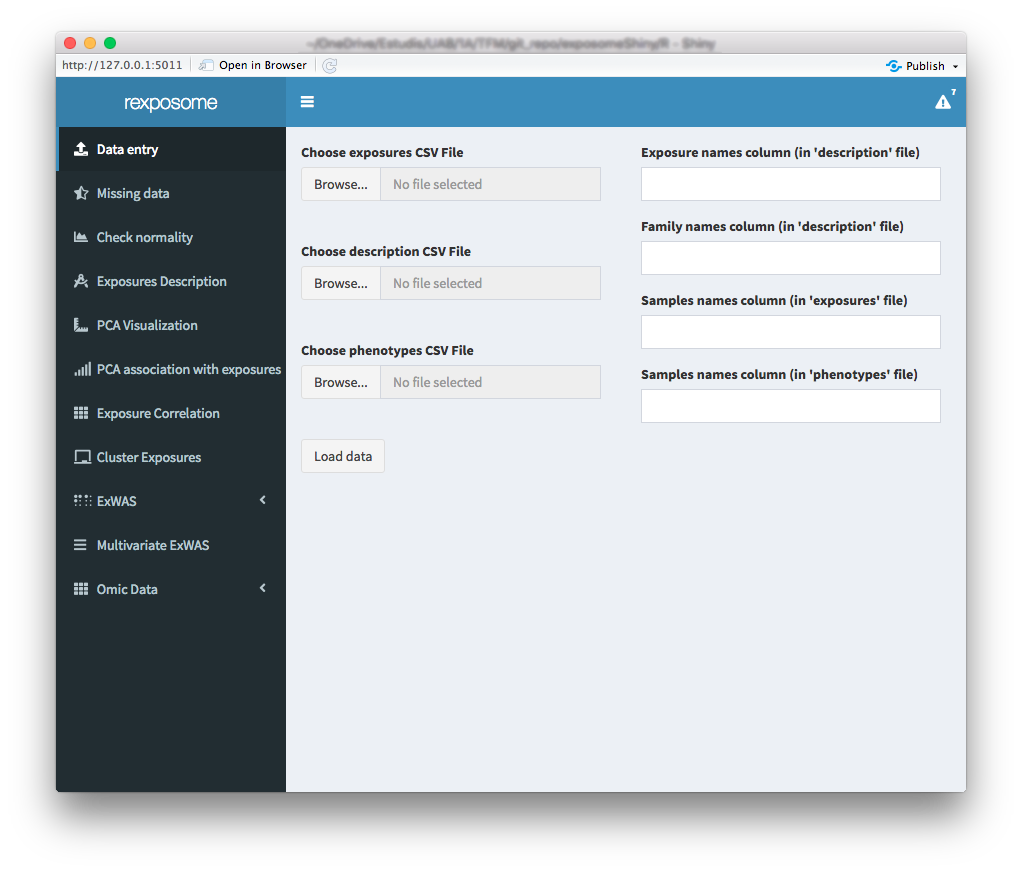
\includegraphics{images/analysis1_2.png}
If exposomeShiny detects LODs (limit of detection) on the exposures file (exposures with value: -1), it will prompt the table with the exposures with LOD and double clicking on the desired cell will enable edit mode to input the instrument LOD. There's also the option of selecting ``Random imputation'' on the imputation method in order to imputate with random values instead of LOD/sqrt(2).

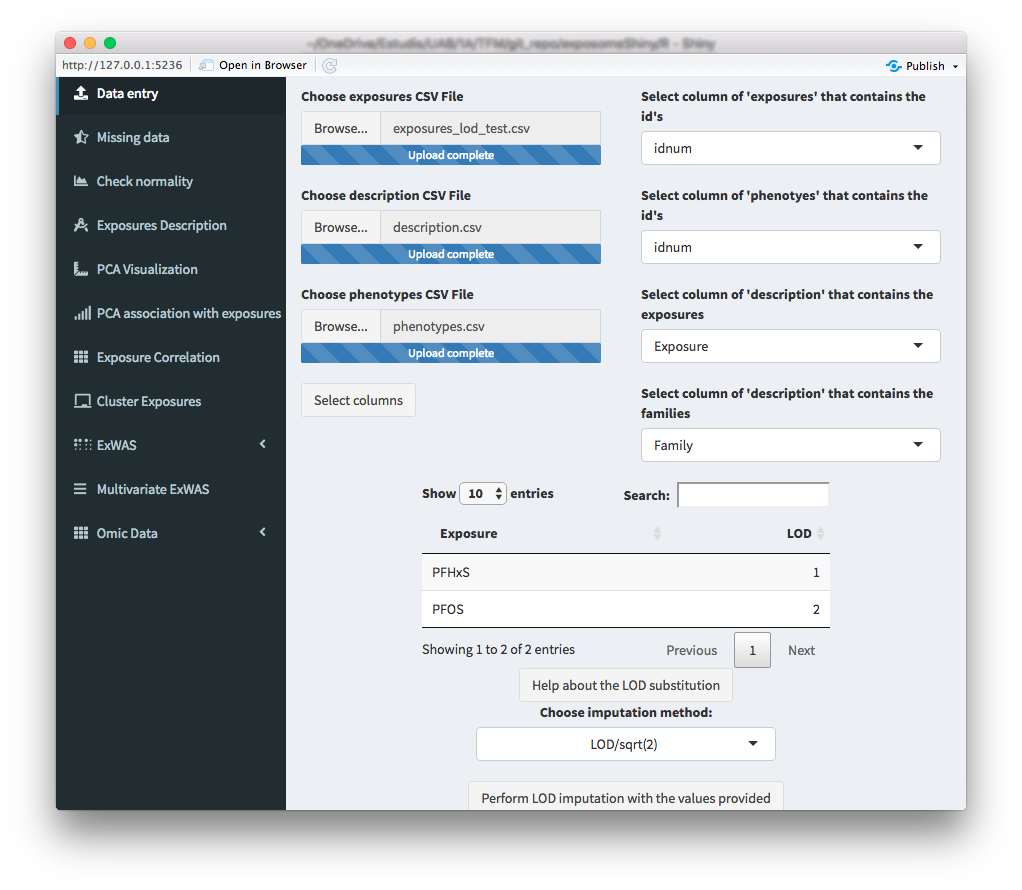
\includegraphics{images/analysis1_3.png}

\hypertarget{missing-imputation}{%
\subsection{Missing imputation}\label{missing-imputation}}

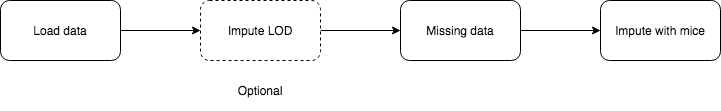
\includegraphics{images/analysis2_1.png}

Once the dataset is loaded into the Shiny, look at the ``Missing Data'' tab to check the percentages of missing data for each exposure present.

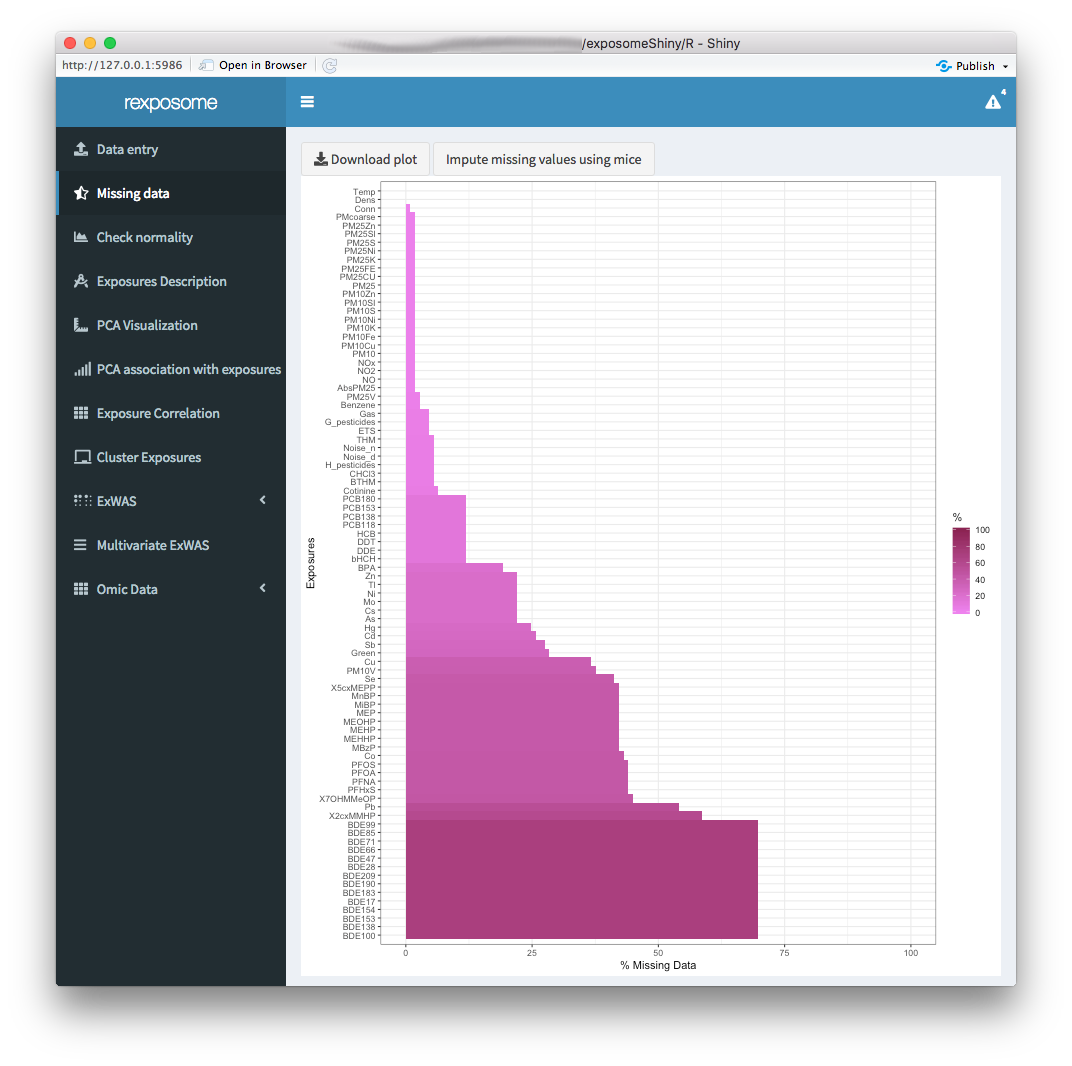
\includegraphics{images/analysis2_2.png}

To impute the missing values select ``Impute missing values using mice''. After the process finishes, the expect output should be a new missing data graph where there's no missing of any exposure.

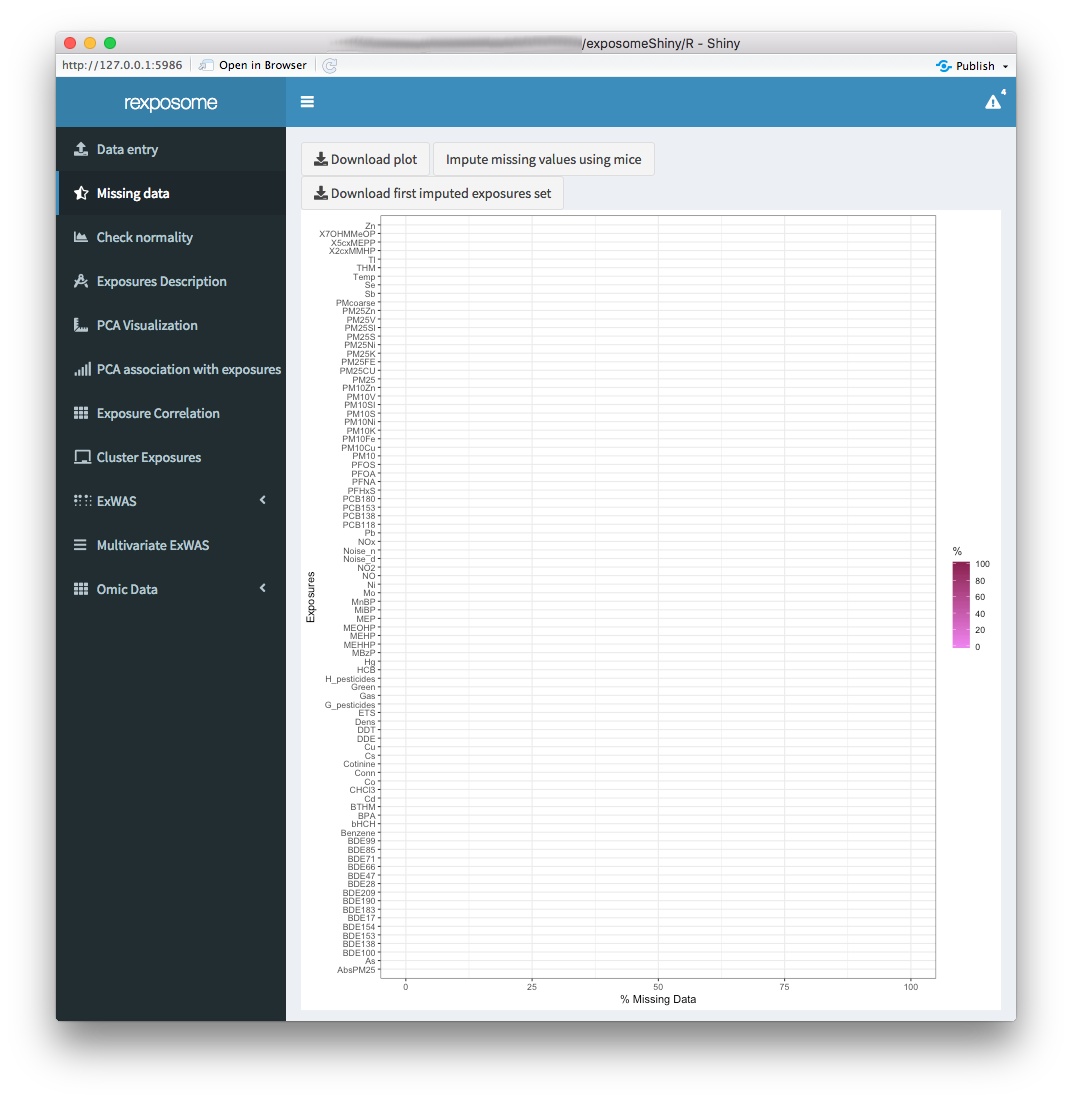
\includegraphics{images/analysis2_3.png}
The new imputed exposures set can be downloaded as a \texttt{*.csv} file, please note that the downloaded file just assigns numbers to the \texttt{idnum} column, if the data you are using has different \texttt{idnum} format it's needed to format it properly so that it matches the \texttt{idnum} on the phenotypes input file when inputting it to the Shiny.

\hypertarget{normality-correction}{%
\subsection{Normality correction}\label{normality-correction}}

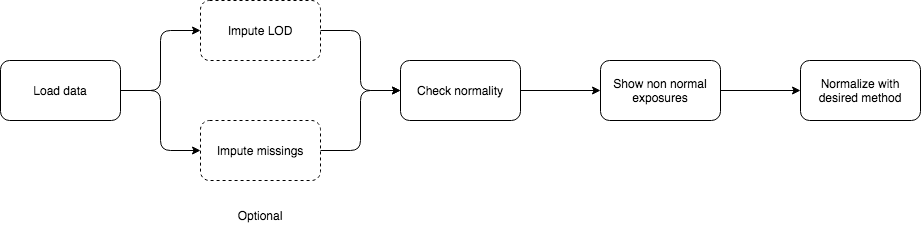
\includegraphics{images/analysis3_1.png}

Once the dataset is loaded into the Shiny, look at the ``Check Normality'' tab to check which exposures are not normal (Normality = false). By selection from the table the desired exposure and clicking the ``Plot histogram of selected exposure'', as the label of the button implies, a histogram of the selected exposure from the table can be seen.

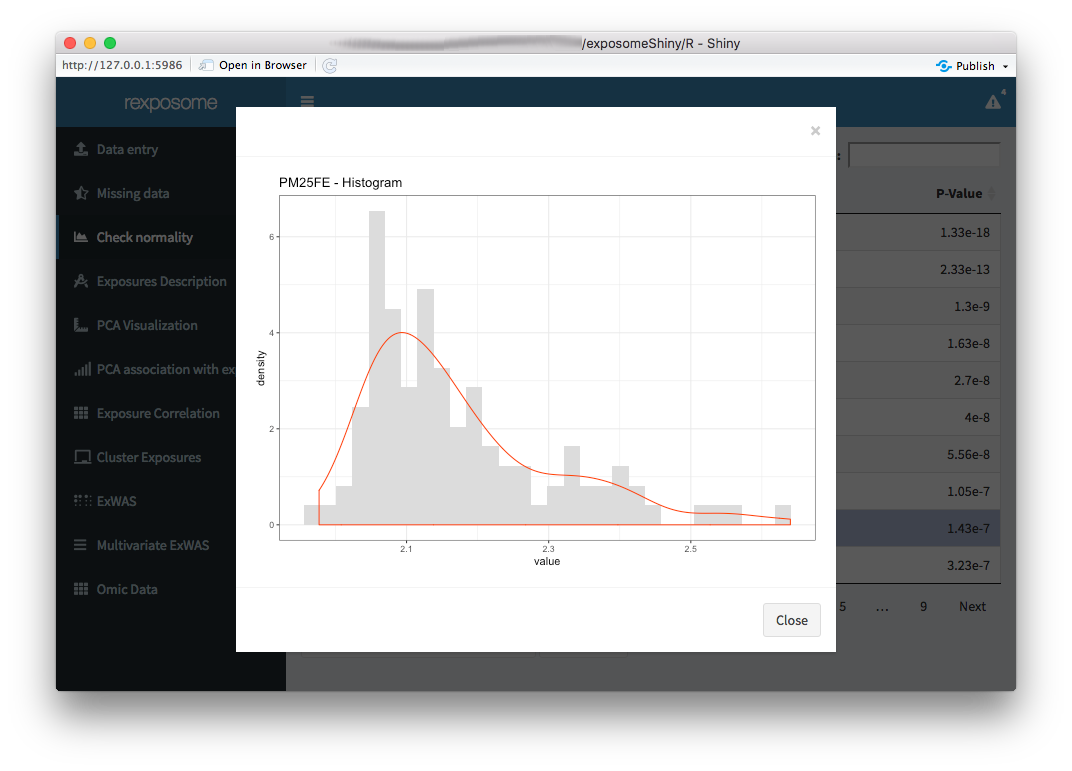
\includegraphics{images/analysis3_2.png}

By clicking the ``Show false'' button, all the non normal exposures are listed with the method that will be applied to normalize, this table can be edited (the ``Normalization method'' column) by double clicking on the desired row. There are three possible methods to use, ``log'' (default), ``\^{}1/3'' and ``sqrt''. If no method is desired to be applied to an exposure input ``none''.

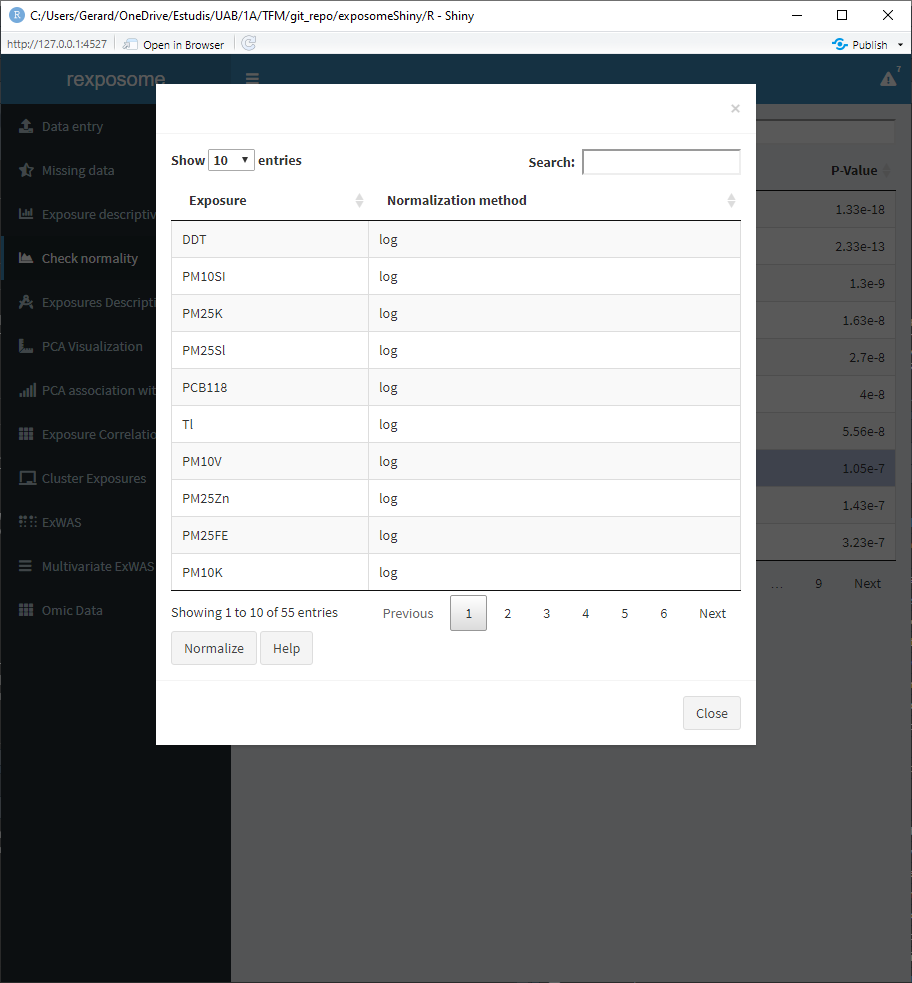
\includegraphics{images/analysis3_3.png}

Click ``Normalize'' and the normalization method selected will be applied, the table on the ``Check Normality'' tab will be updated with the results of the normalization.

\hypertarget{exposures-description}{%
\subsection{Exposures description}\label{exposures-description}}

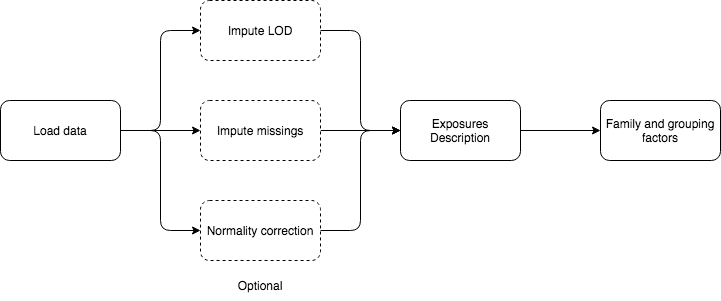
\includegraphics{images/analysis4_1.png}

To see all the insights of the exposures dataset loaded into the Shiny, once loaded it check the exposures description tab, there are three options to dig into the dataset, the family (family of the exposure) to visualize and two grouping factors (phenotypes).

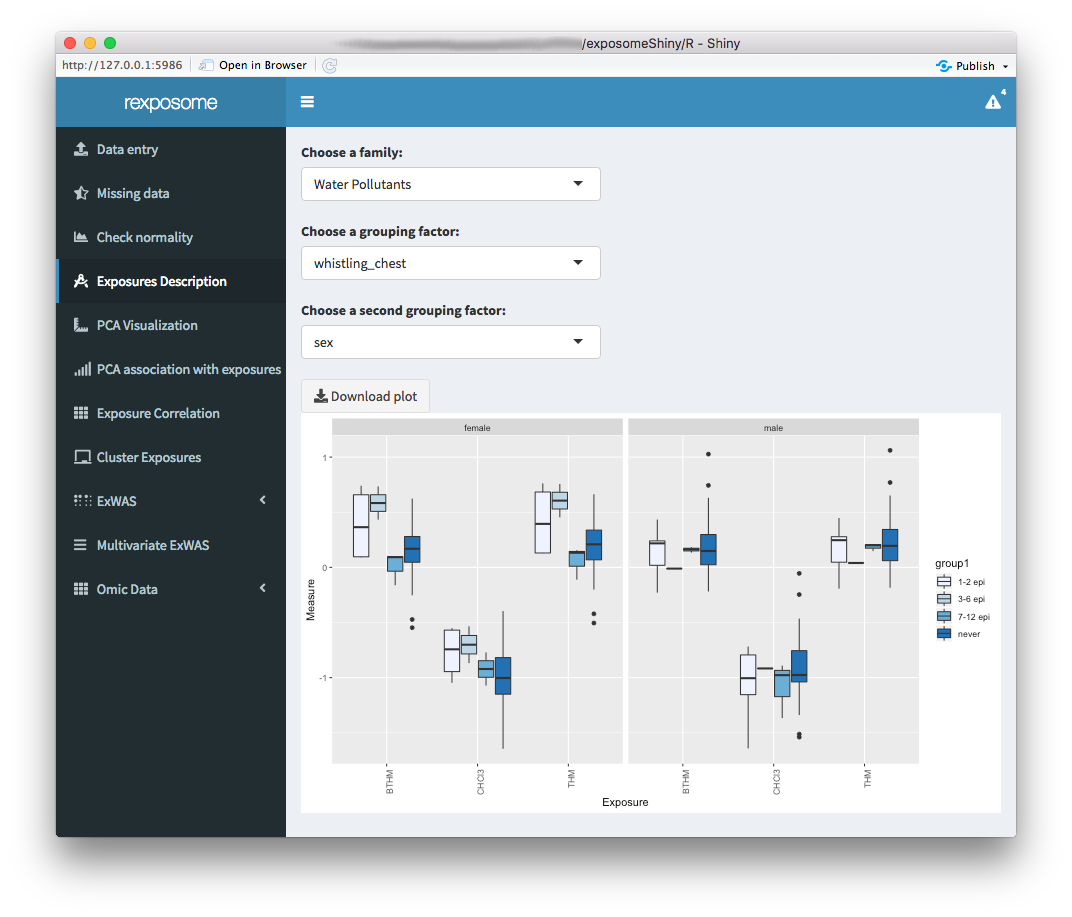
\includegraphics{images/analysis4_2.png}

\hypertarget{pca-analysis}{%
\subsection{PCA Analysis}\label{pca-analysis}}

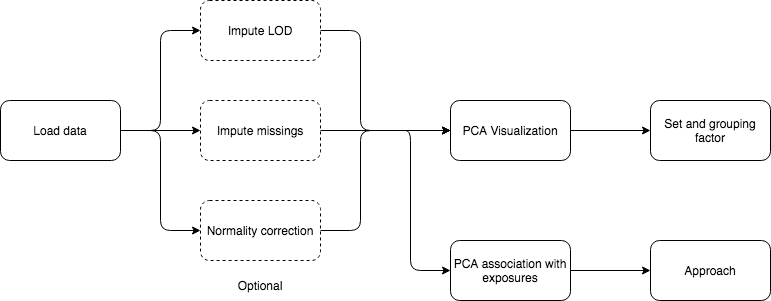
\includegraphics{images/analysis5_1.png}

To see the results of a PCA (principal component analysis) study, load the data and check the PCA Visualization tab, there a set and grouping factor can be choose, it's important noting (as it's already stated on the Shiny) that the grouping parameter only works when the set is selected to ``samples''.

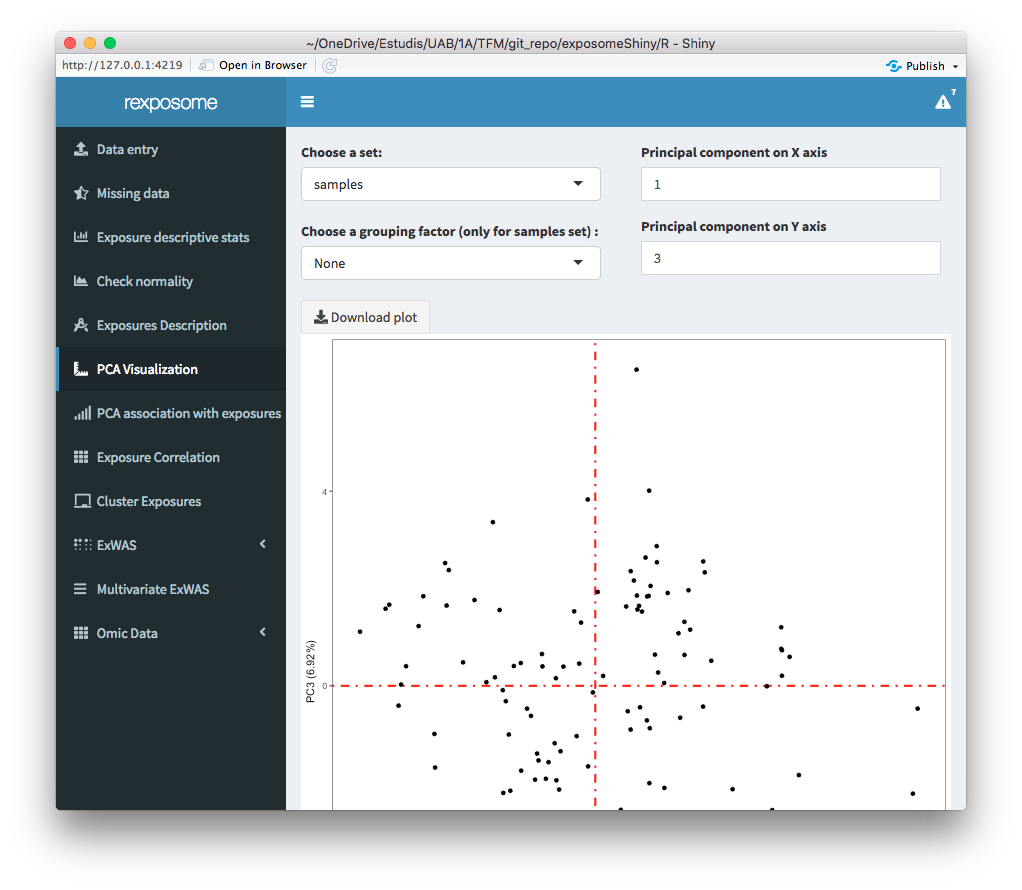
\includegraphics{images/analysis5_2.png}

If the association of the PCA analysis with the exposures is desired to visualize, check the ``PCA association with exposures'' tab, there are two grouping methods to visualize, the phenotypes to principal components and the exposures to principal components.

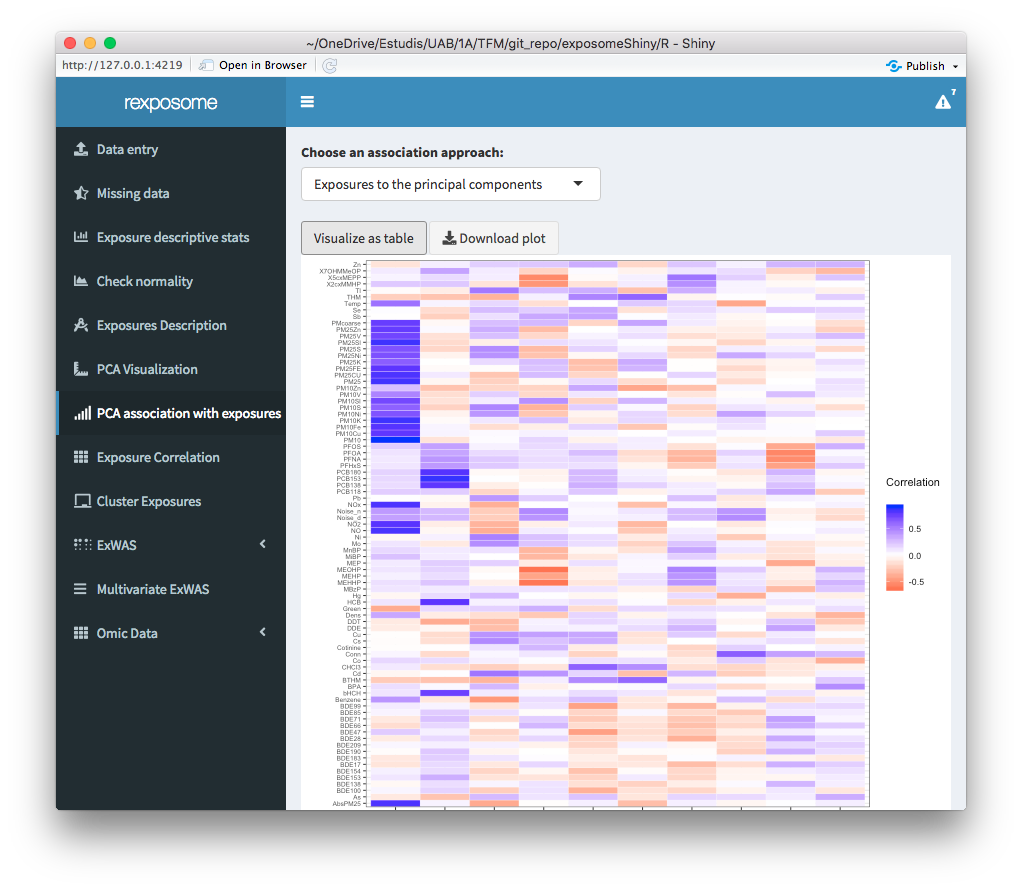
\includegraphics{images/analysis5_3.png}

\hypertarget{clusterization-and-correlation-of-exposures}{%
\subsection{Clusterization and correlation of exposures}\label{clusterization-and-correlation-of-exposures}}

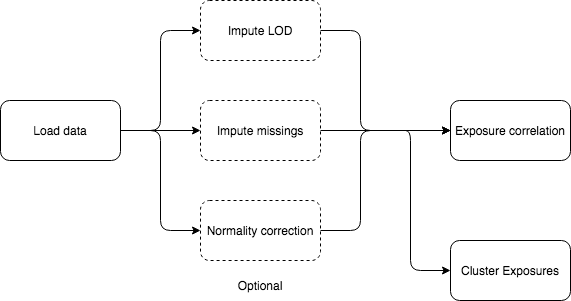
\includegraphics{images/analysis6_1.png}

To see the results of the exposure correlation and clustering, select the corresponding tab to each analysis. For the exposure correlation analysis there are two visualizations, the matrix representation and the circos.

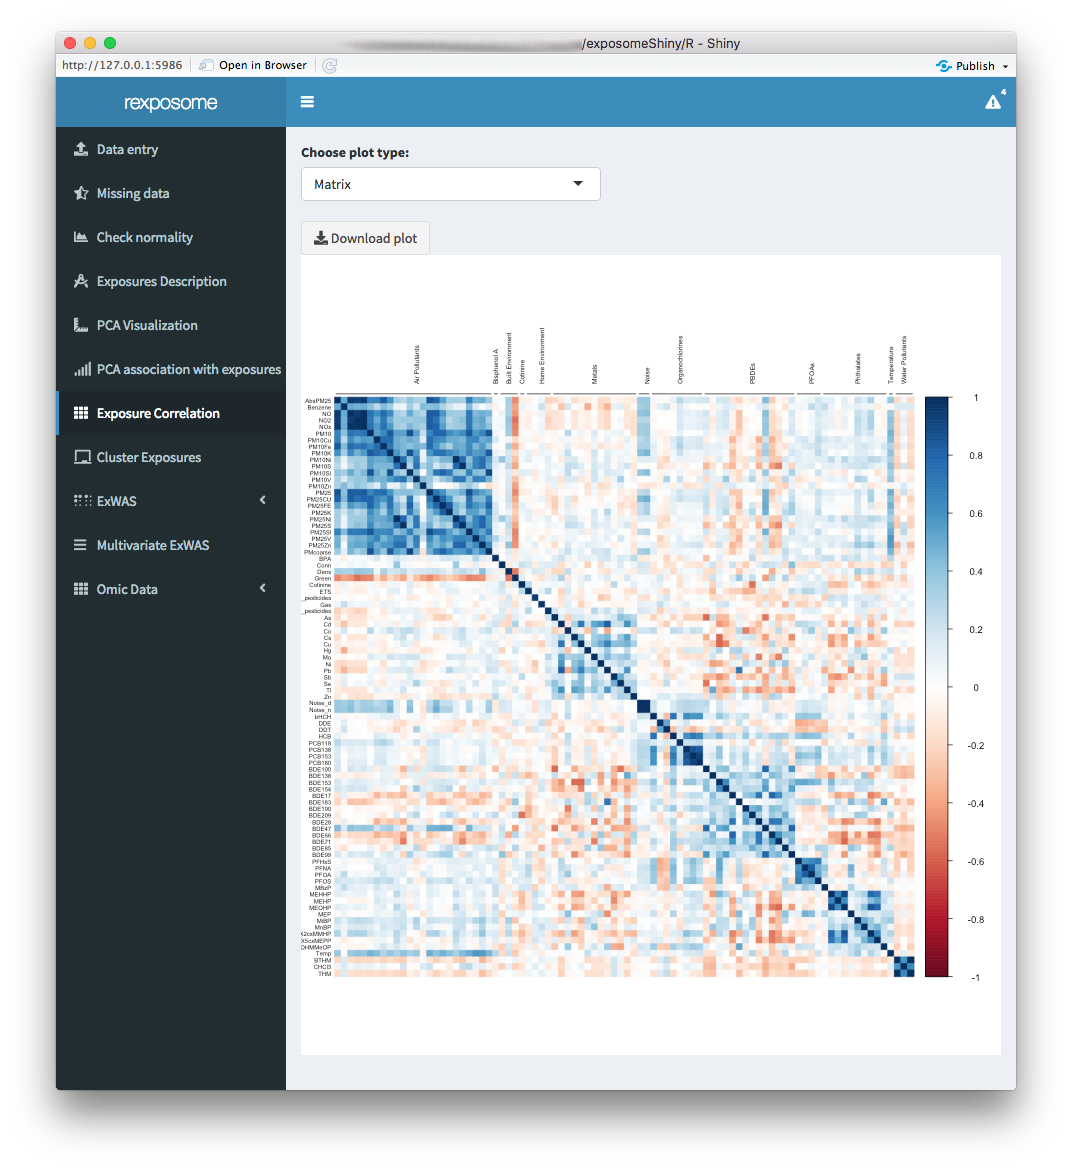
\includegraphics{images/analysis6_2.png}

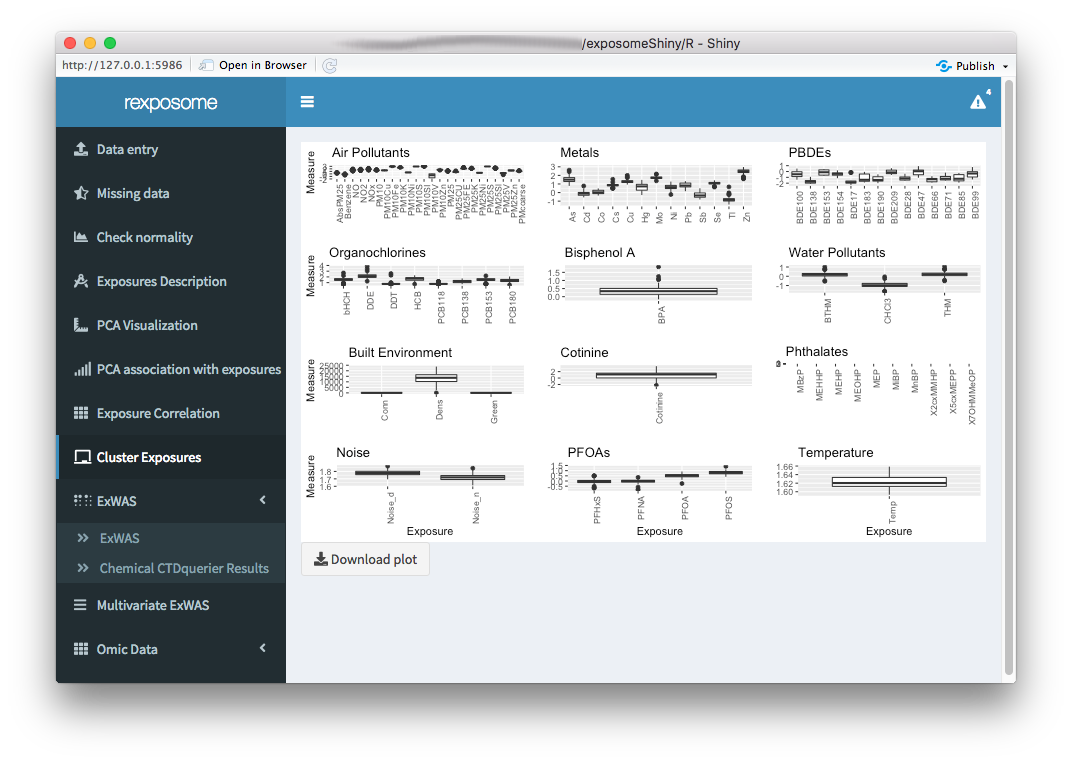
\includegraphics{images/analysis6_3.png}

\hypertarget{exwas}{%
\subsection{ExWAS}\label{exwas}}

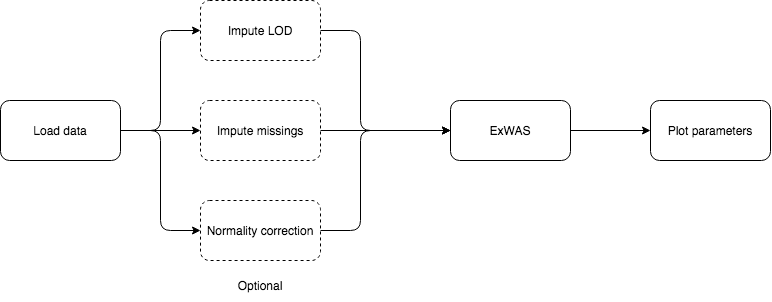
\includegraphics{images/analysis7_1.png}

To perform an ExWAS (exposome-wide association) study, check the ExWAS tab and select the addecuate parameters for the ExWAS plot, there are two different plot representations, the output variable to choose (phenotype), the output family and as many covariables (phenotypes) as the user wants. There are internal checks to advise the user on which parameters to select depending if the selected outcome is numerical or bionomial.

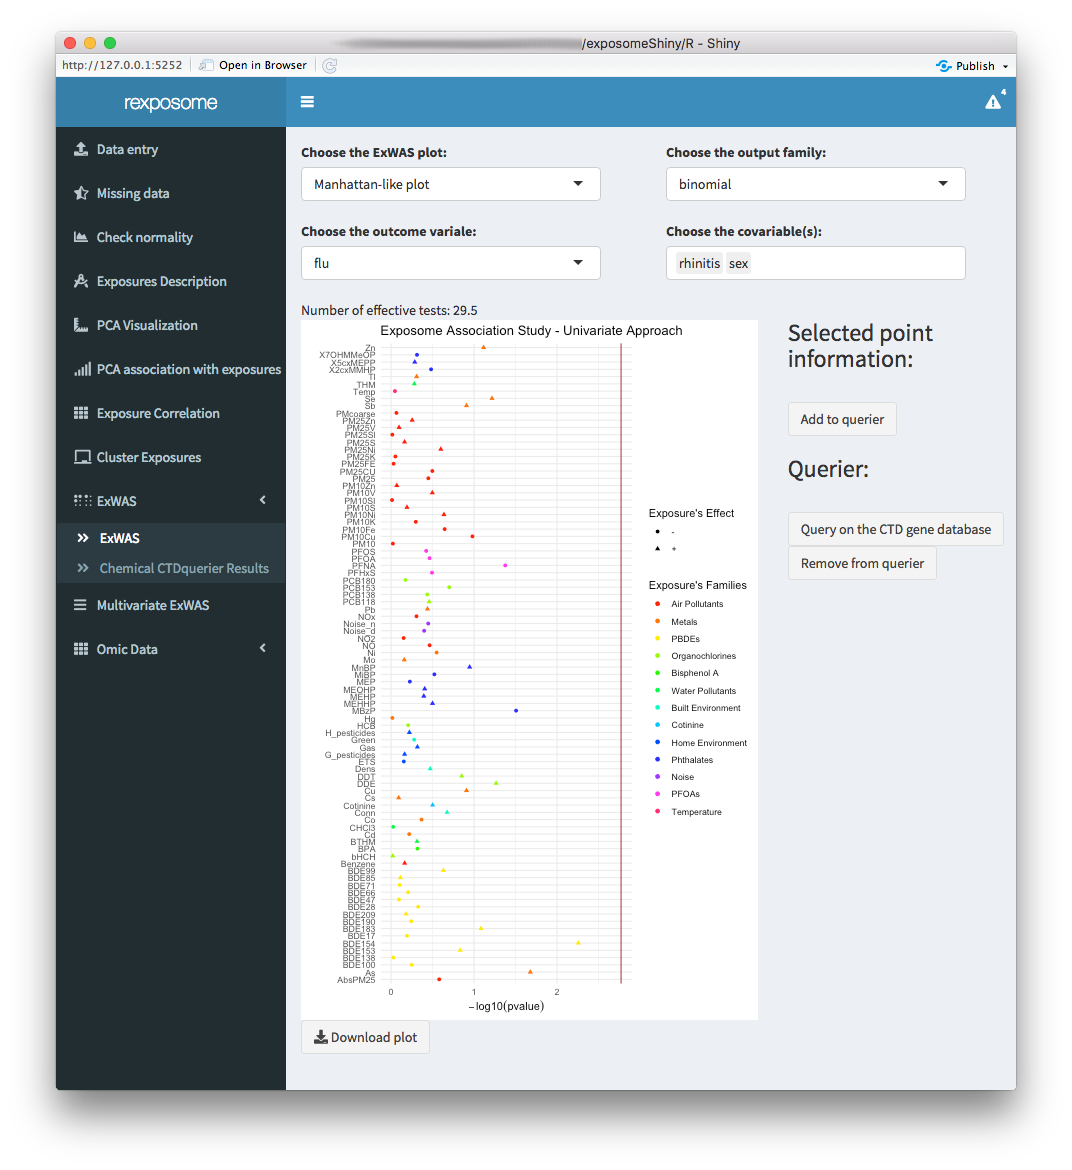
\includegraphics{images/analysis7_2.png}

\hypertarget{exwas---ctdquerier}{%
\subsection{ExWAS - CTDquerier}\label{exwas---ctdquerier}}

The ExWAS tab also is able to perform a CTD query of the desired chemicals.

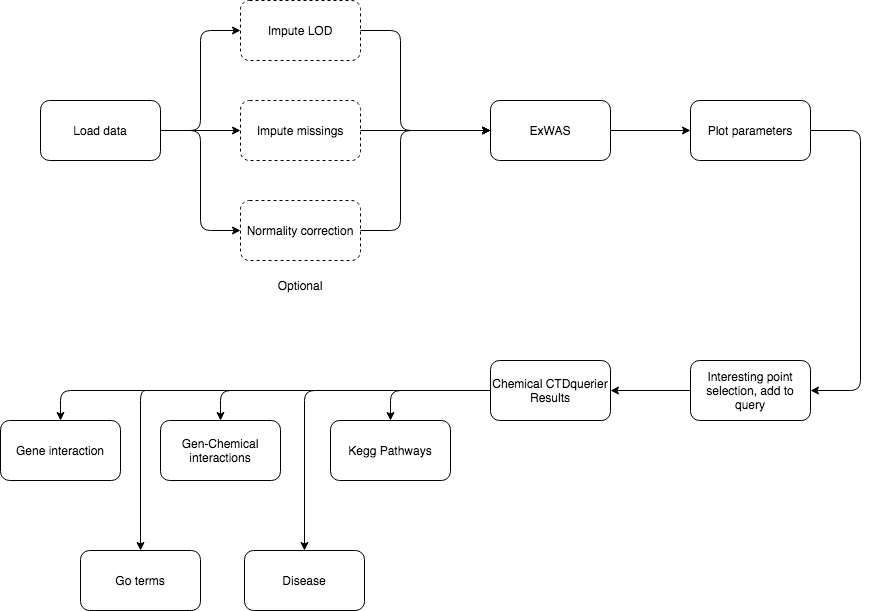
\includegraphics{images/analysis7_3.png}

To perform a CTDquerier of chemicals with the results of the ExWAS, click on the desired exposure to preload it into the query, when clicked, a chemical name with it's associated P-Value will appear on the table on the right, if that's the desired chemical to add to the query list click ``Add to querier''. In the case of adding an unwanted chemical to the query list, select it (or them) by clicking on the Querier list and click on ``Remove from querier''.

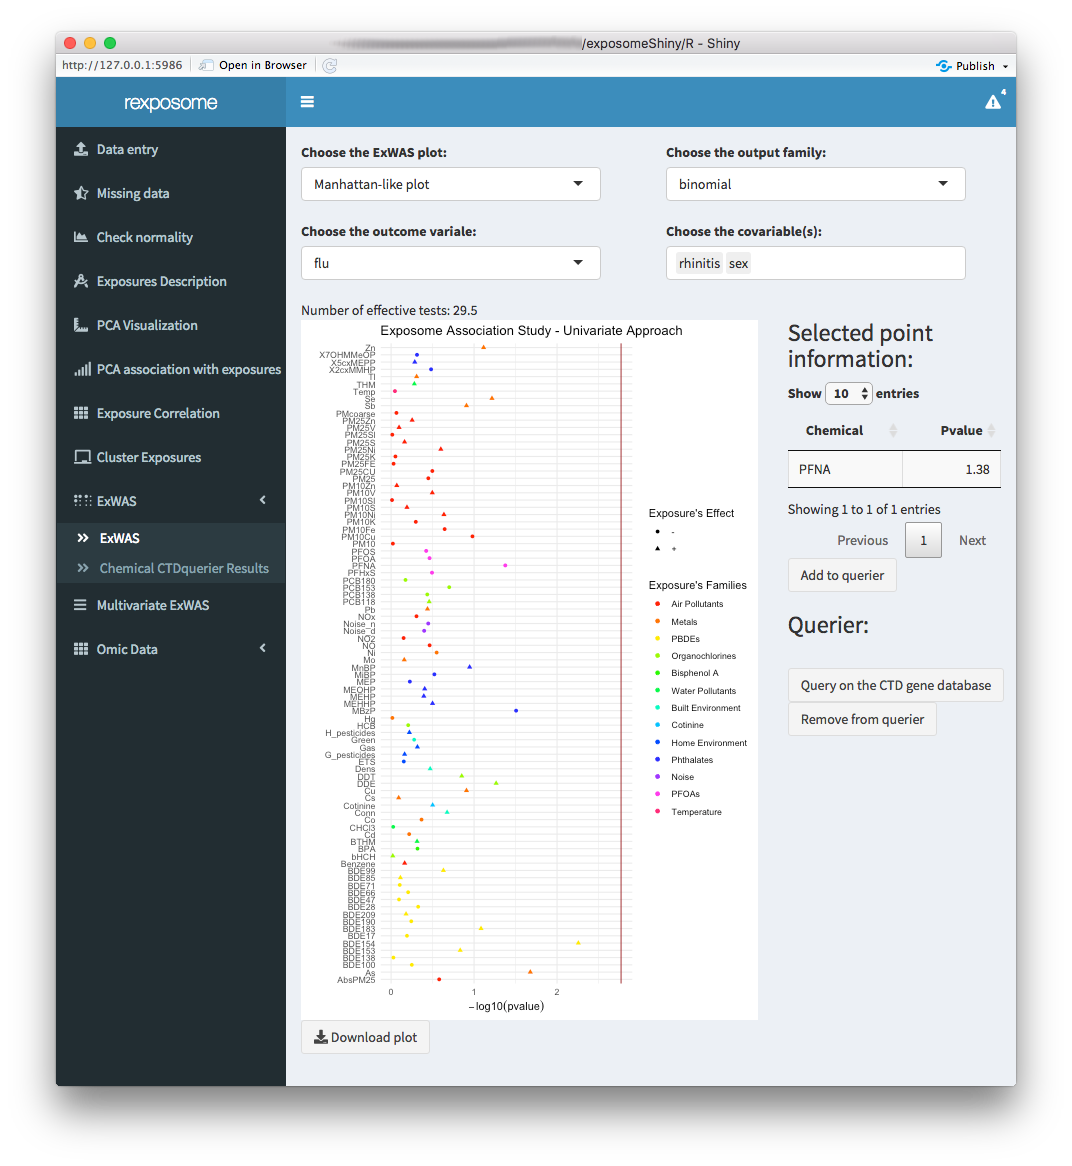
\includegraphics{images/analysis7_4.png}

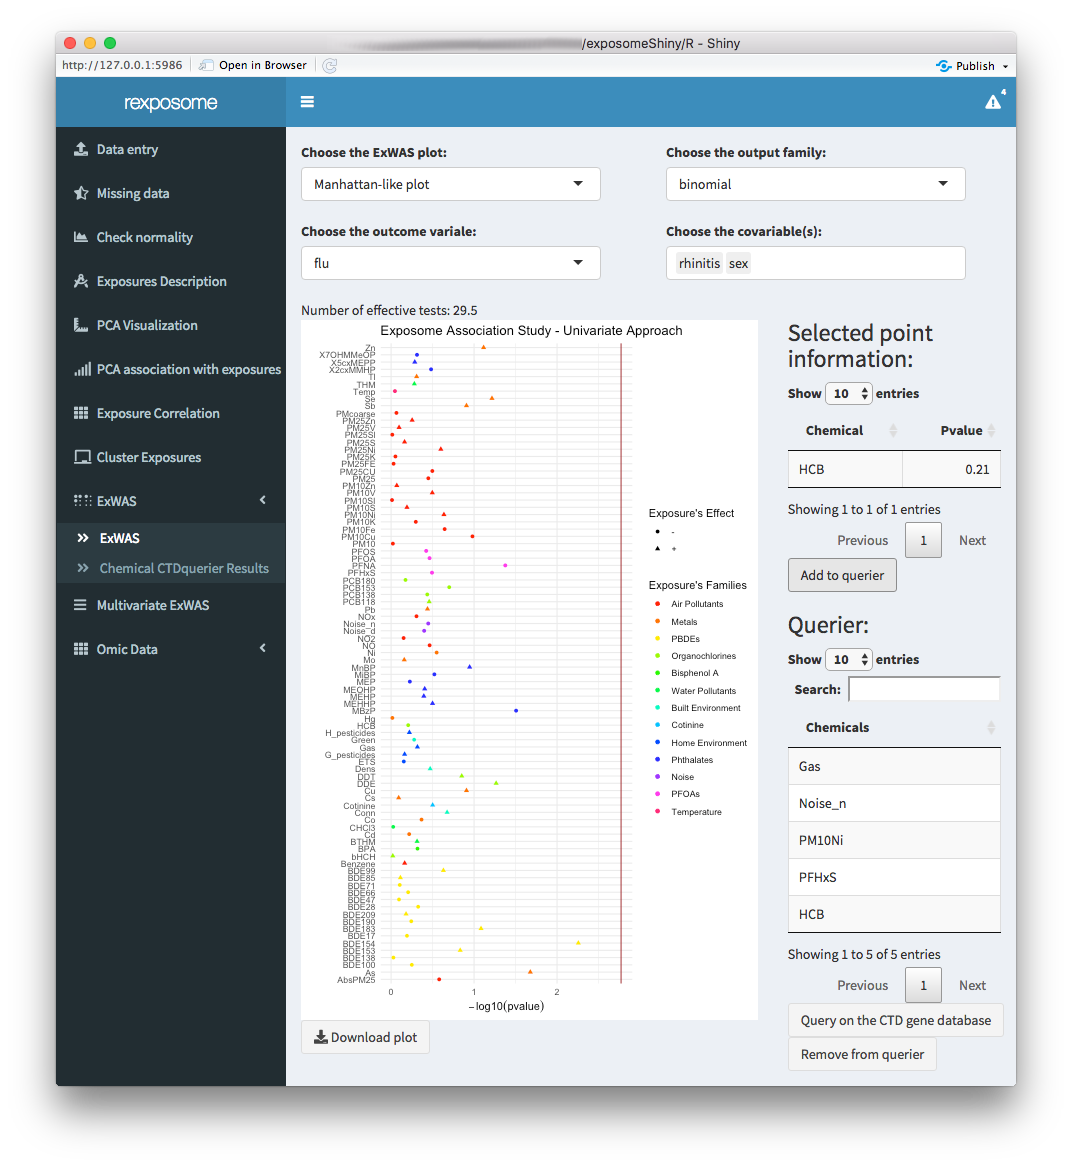
\includegraphics{images/analysis7_5.png}

To do the query of the chemicals to de CTD database click on ``Query on the CTD gene database'' and see the results on the ``Chemical CTDquerier Results'' subtab. It's important noting that on the ``Kegg pathways'' and ``Go terms'' the input field corresponds to the negative exponent of the filter.

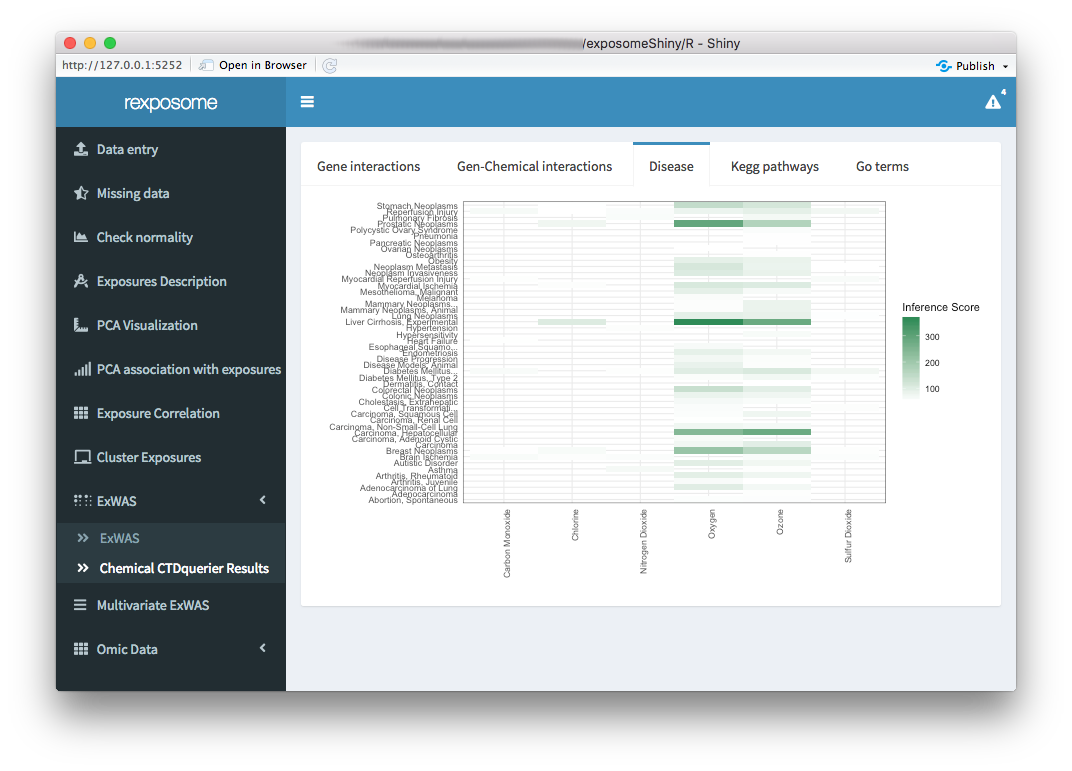
\includegraphics{images/analysis7_6.png}

\hypertarget{multivariate-exwas}{%
\subsection{Multivariate ExWAS}\label{multivariate-exwas}}

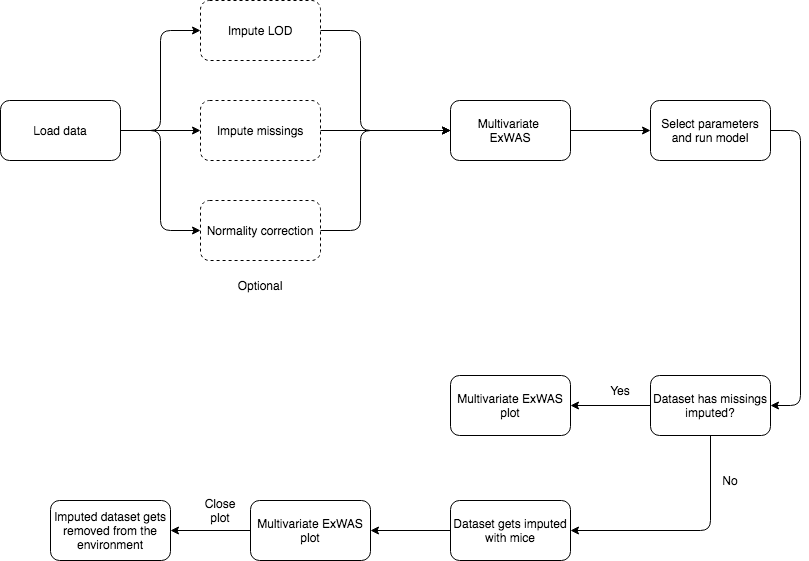
\includegraphics{images/analysis8_1.png}

To perform a multivariate ExWAS study, check the Multivariate ExWAS tab and select the desired output parameter, click on run model to generate the plot. As on the ExWAS plot options there's implemented an internal check to advise the user on which parameters to select depending if the selected outcome is numerical or bionomial, as the diagrams states if the dataset has not been imputed the missings, it will automatically do it to perform the Multivariate ExWAS, however when closing the plot the imputed dataset will be removed from the environment, so all the other studies performed afterwards will not be altered.

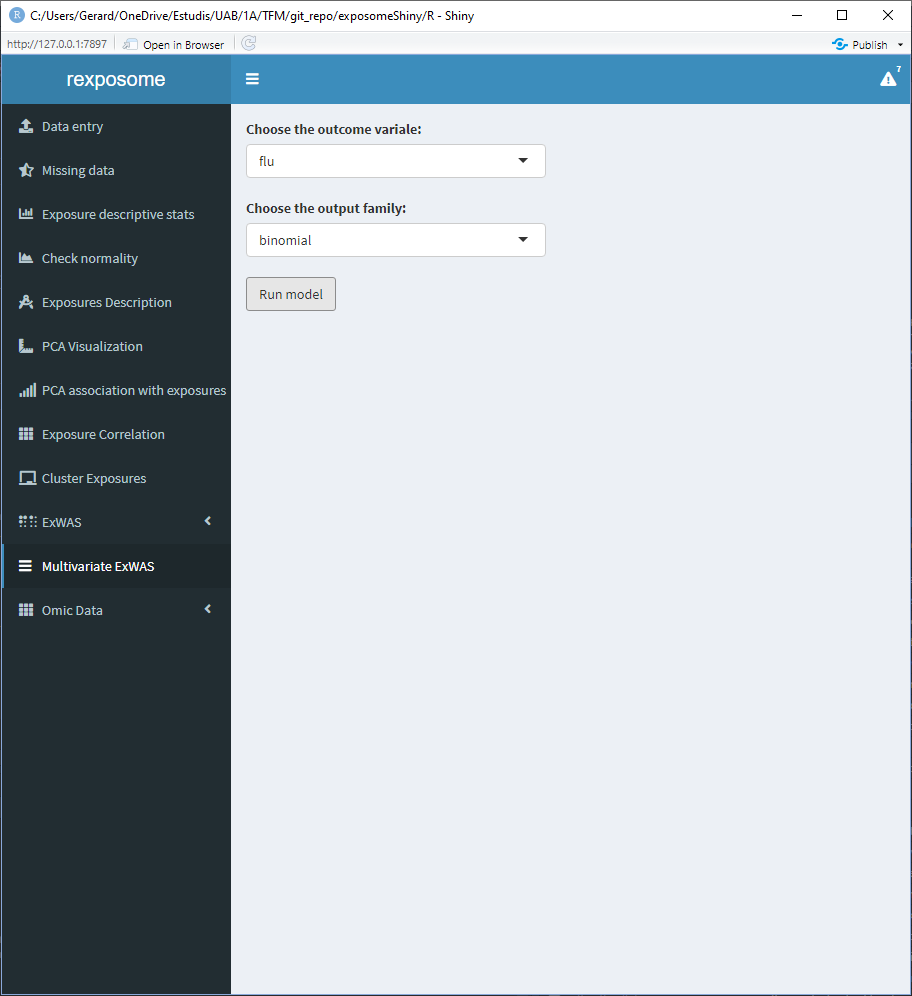
\includegraphics{images/analysis8_2.png}
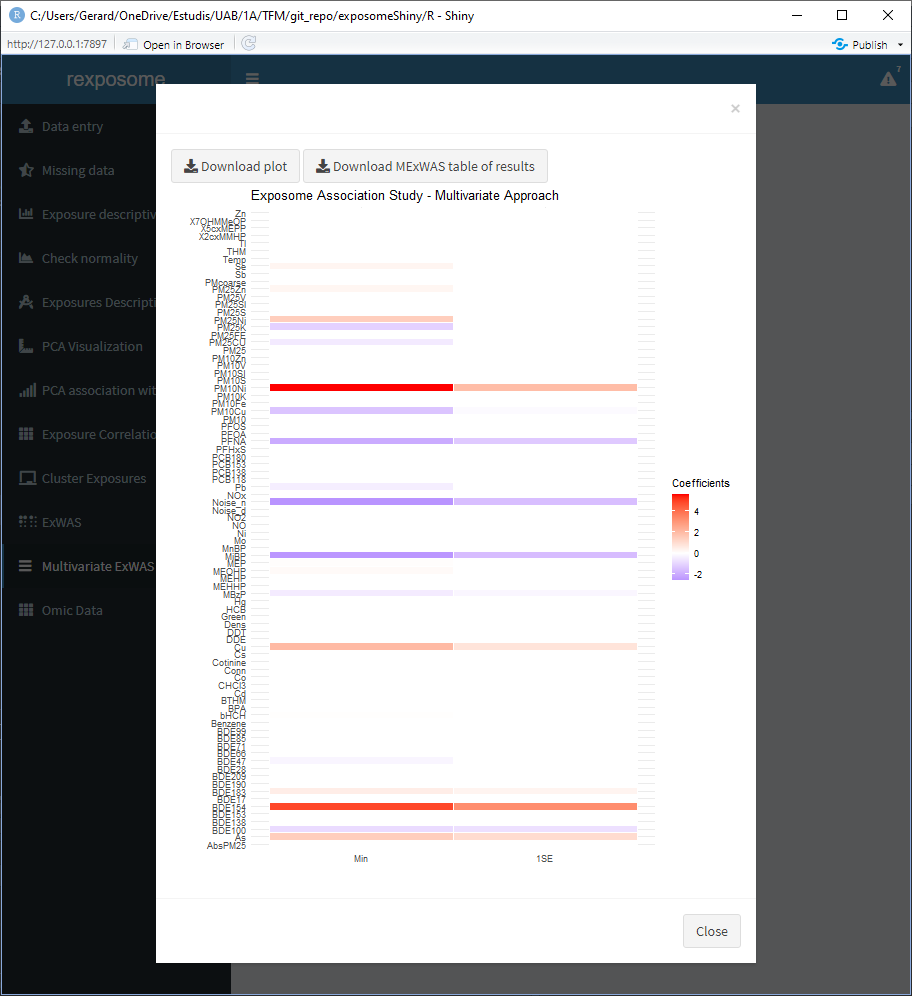
\includegraphics{images/analysis8_3.png}

\hypertarget{exposome-omic-analysis}{%
\section{Exposome-Omic analysis}\label{exposome-omic-analysis}}

It's important noting that the maximum size of the omics data is 30 MB, if the omics file to be analyzed is bigger, change the line number 2 of the \texttt{server.R} file.

\begin{Shaded}
\begin{Highlighting}[]
  \CommentTok{# the "30" refers to 30MB, change as needed}
\KeywordTok{options}\NormalTok{(}\DataTypeTok{shiny.maxRequestSize=}\DecValTok{30}\OperatorTok{*}\DecValTok{1024}\OperatorTok{^}\DecValTok{2}\NormalTok{)}
\end{Highlighting}
\end{Shaded}

\hypertarget{association-analysis}{%
\subsection{Association analysis}\label{association-analysis}}

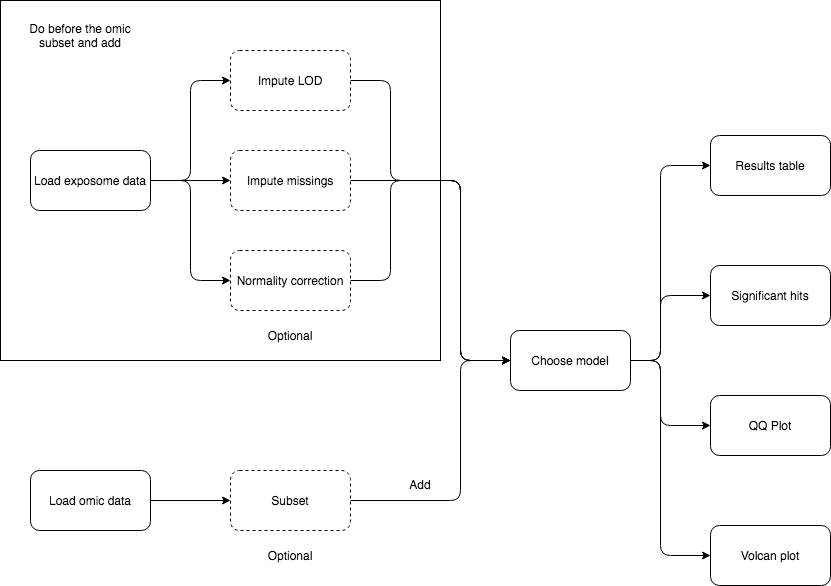
\includegraphics{images/analysis9_1.png}

Do first the proceeding of exposome data load and corresponding treatment if desired, then proceed to load the omic dataset on the ``Data Entry'' subtab of the ``Omic Data'' tab. The omic data should be provided as a \texttt{*.RData} file.

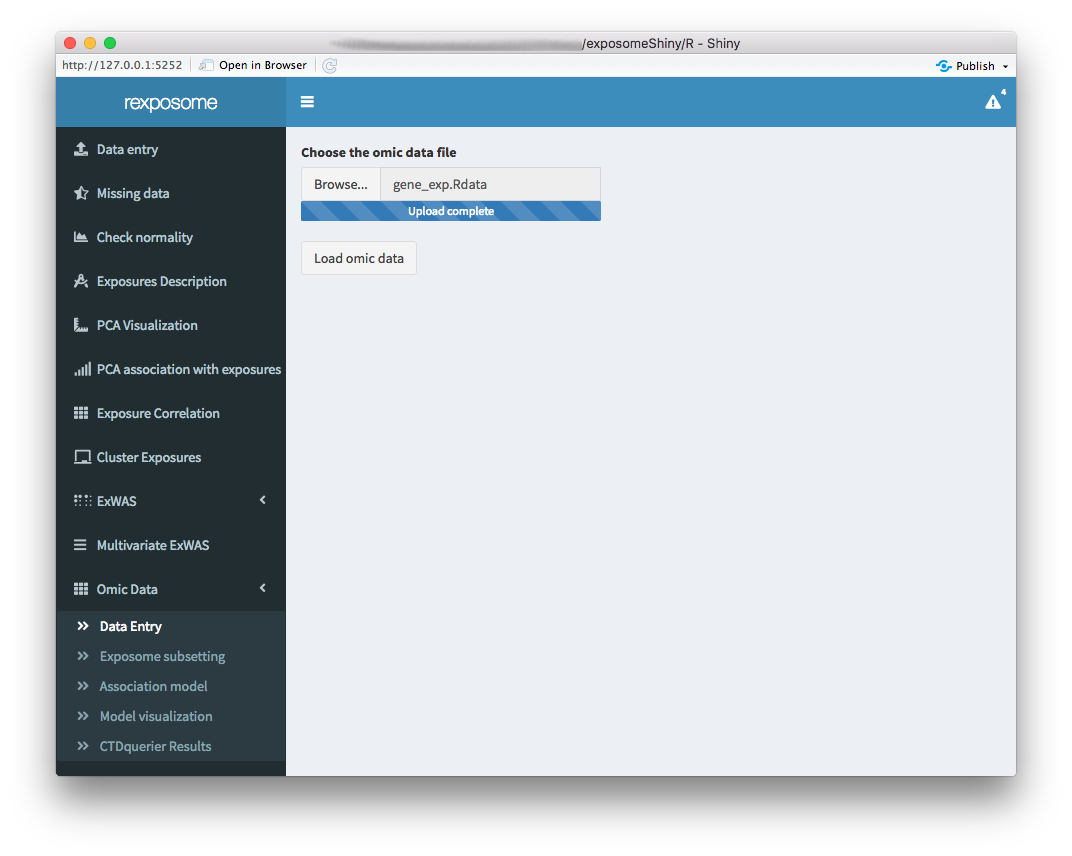
\includegraphics{images/analysis9_2.png}

The exposome dataset can be subseted by families, on the ``Exposome subsetting'' subtab select the families that are desired to be included in this new set to study, if all the families are desired just don't input any and proceed to click the ``Subset and add'', which will trigger the action to combine the subsetted (or not) exposome dataset with the provided omic dataset.

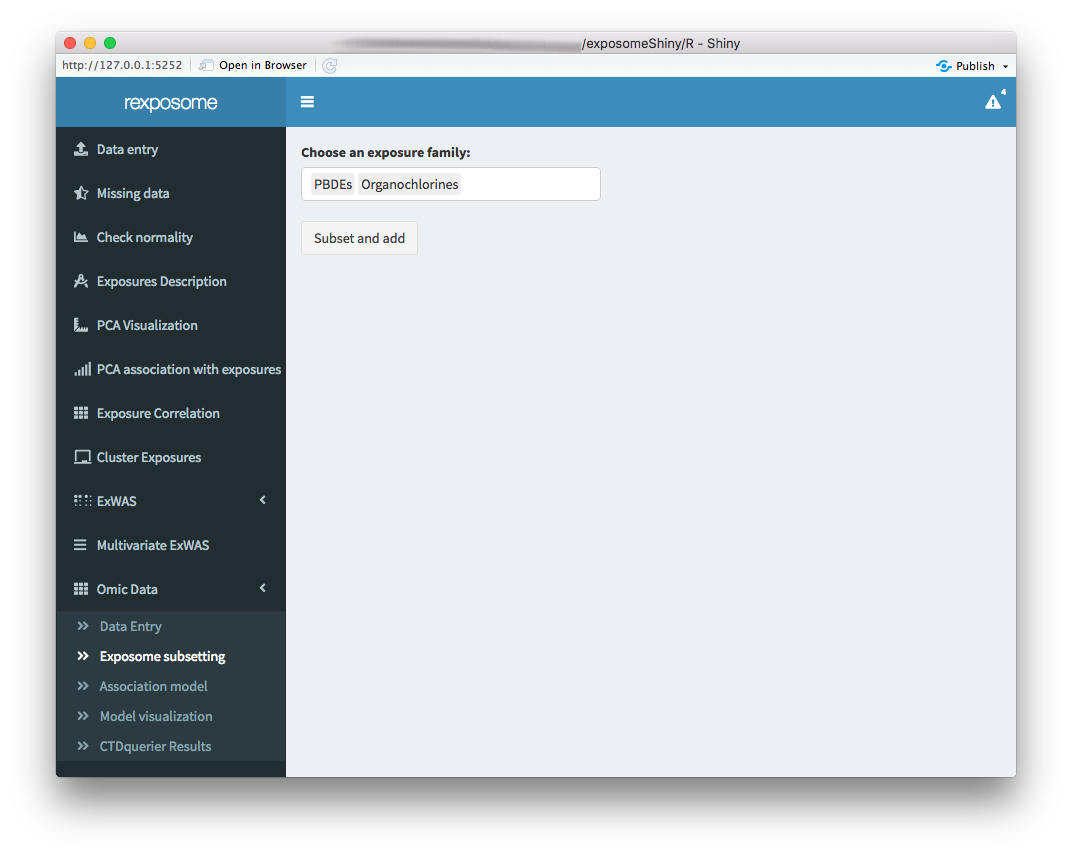
\includegraphics{images/analysis9_3.png}

Select the variables for the association analysis and if SVA is wanted on the ``Association model'' subtab.

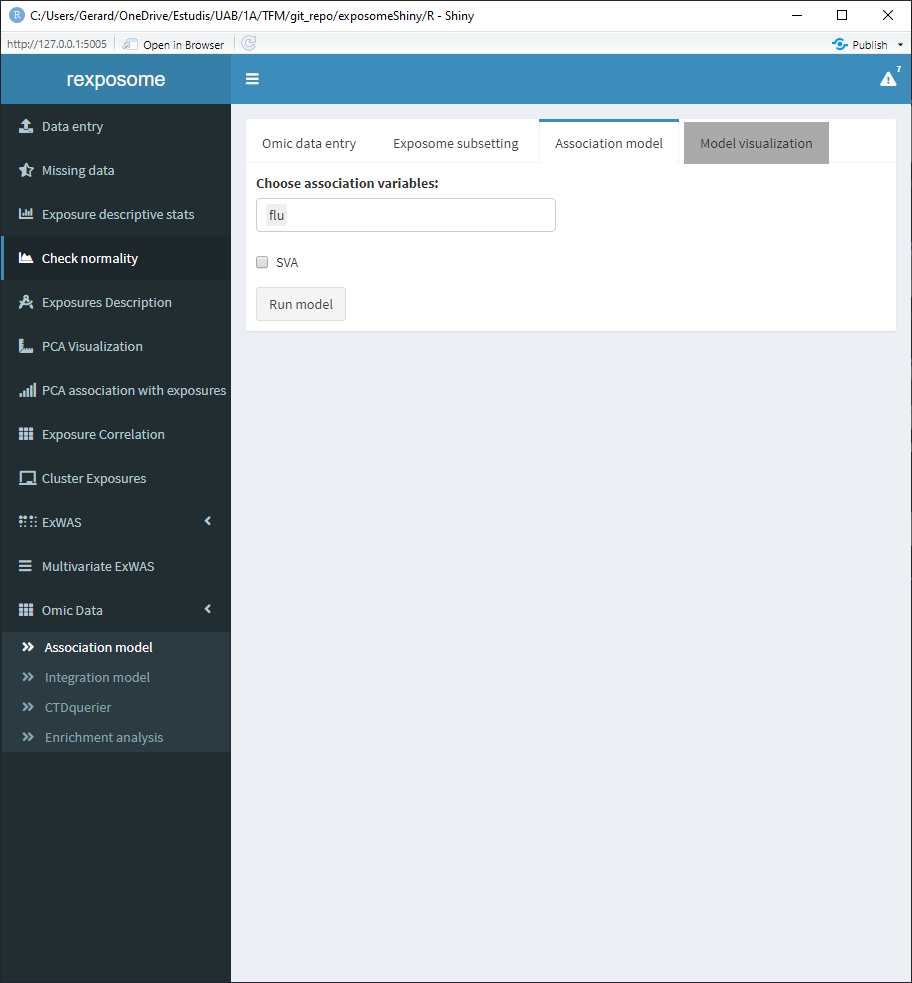
\includegraphics{images/analysis9_4.png}

There are tabs to visualize the results of running the association model, all of the are on the ``Model visualization'' subtab. The ``Results table'' shows the gene, log of the fold change, p-value and adjusted p-value.

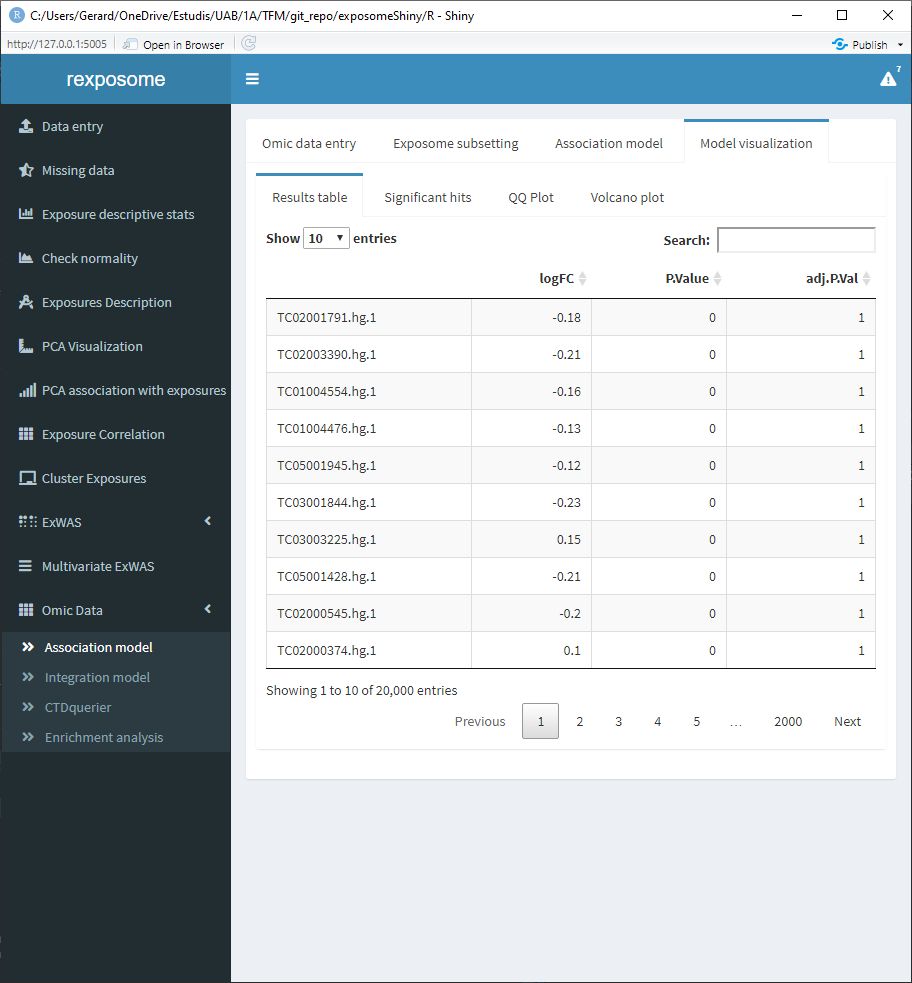
\includegraphics{images/analysis9_5.png}

The ``Significant hits'' shows the exposure, hits and lambda.

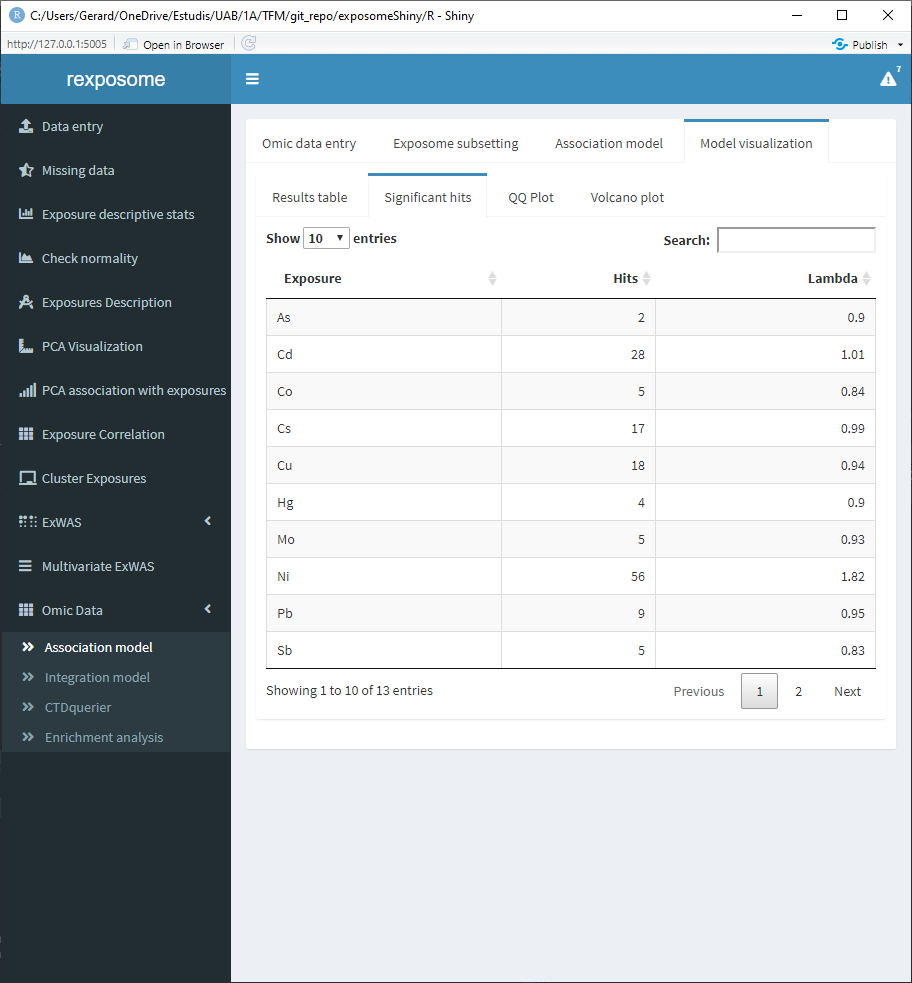
\includegraphics{images/analysis9_6.png}

The QQ Plot shows a QQ plot (expected vs.~observed -lo10(p-value)) for the selected exposure.

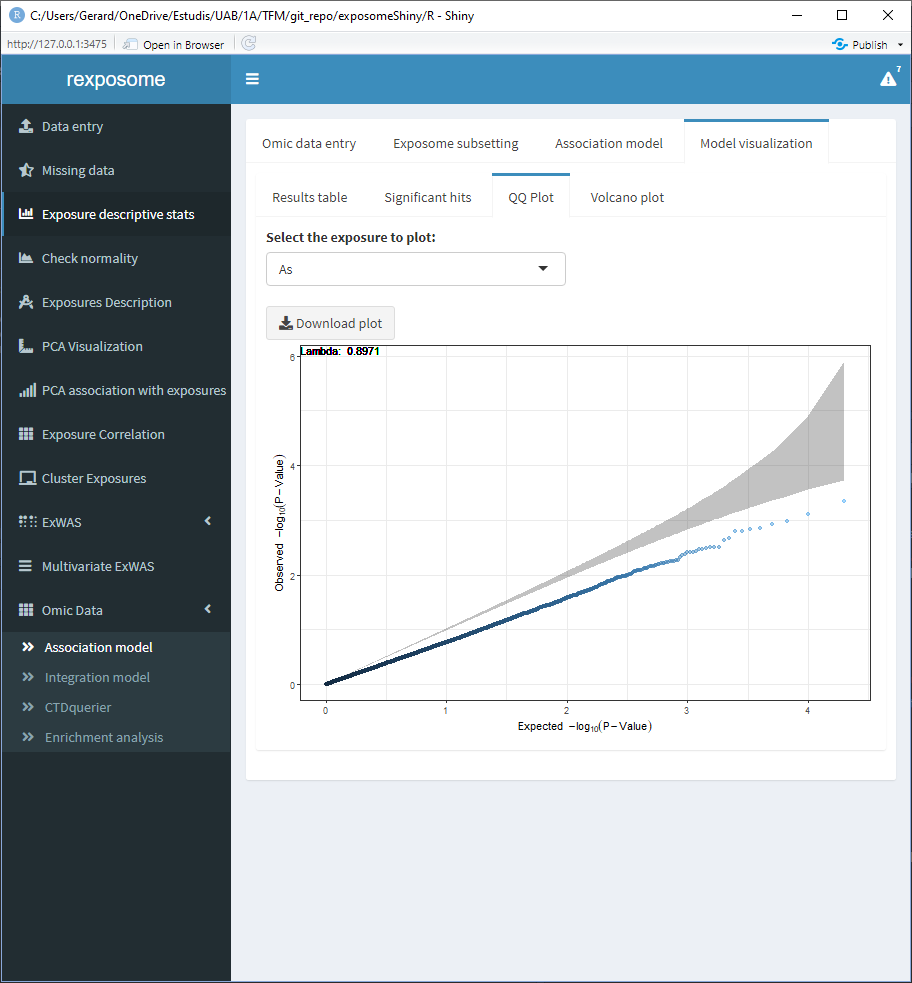
\includegraphics{images/analysis9_7.png}

The Volcan plot shows a volcan plot (log2(fold change) vs -log10(p-value)). For this plot there are two input cells to adjust the horizontal and verital limit lines to filter out the results.

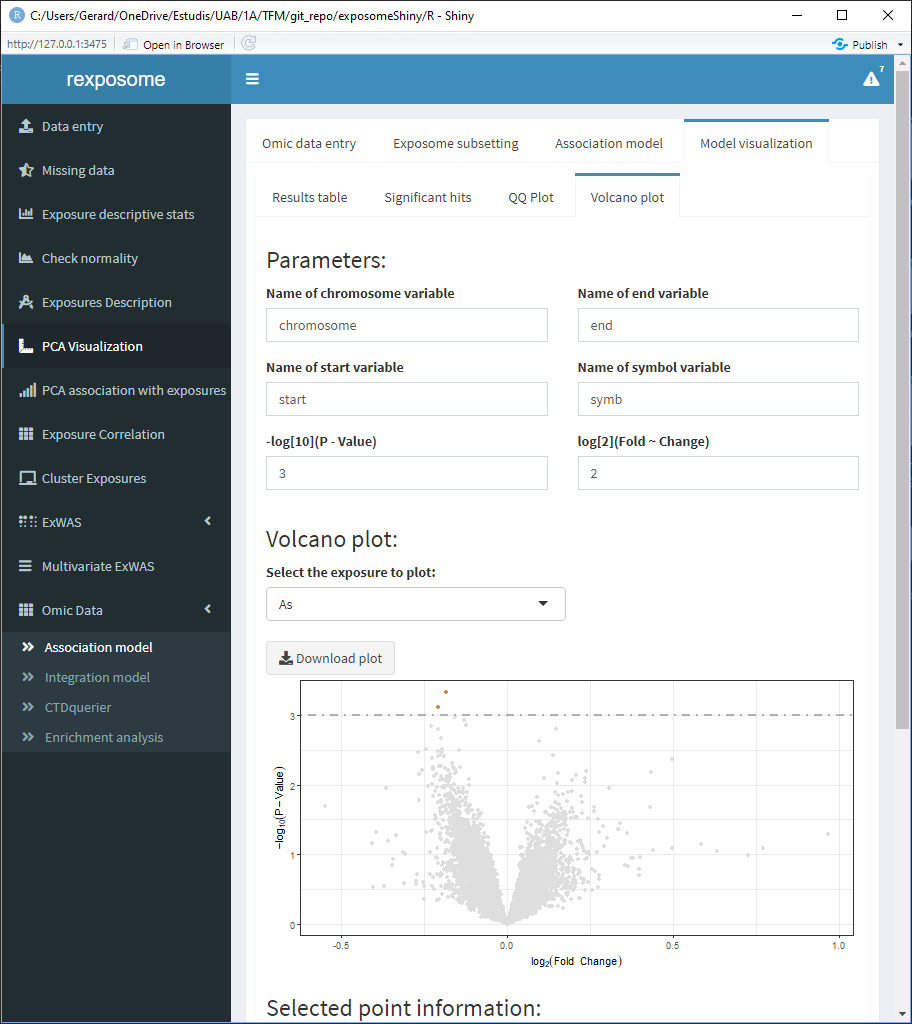
\includegraphics{images/analysis9_8.png}

\hypertarget{ctd-querier}{%
\subsection{CTD querier}\label{ctd-querier}}

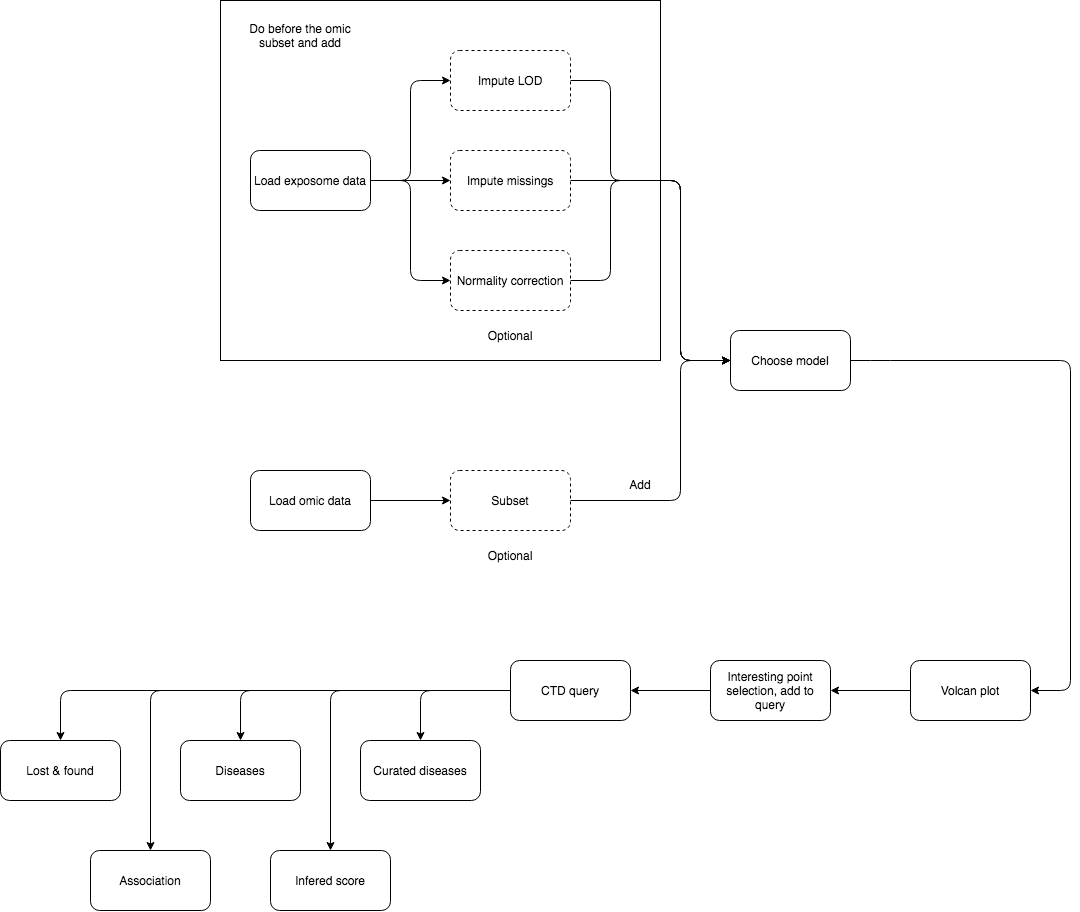
\includegraphics{images/analysis10_1.png}

To perform a CTD querier study of the exposome-omic analysis, as before, load both datasets and run the desired model with them, check the Volcan plot and click on the desired point on the Volcan plot, the information of the selected plot will appear on the table below the plot (sometimes there are many points close so more than one rows can appear on the table), select from the table the desired point to add to the query and click ``Add to querier''. It's important noting that when trying to add to the querier the Shiny will find on the fields of the omic dataset that the user specifies on top of the plot. If the search does not return any symbol a prompt will appear, however if it's found it will be added to the lower table corresponding to the genes to query.

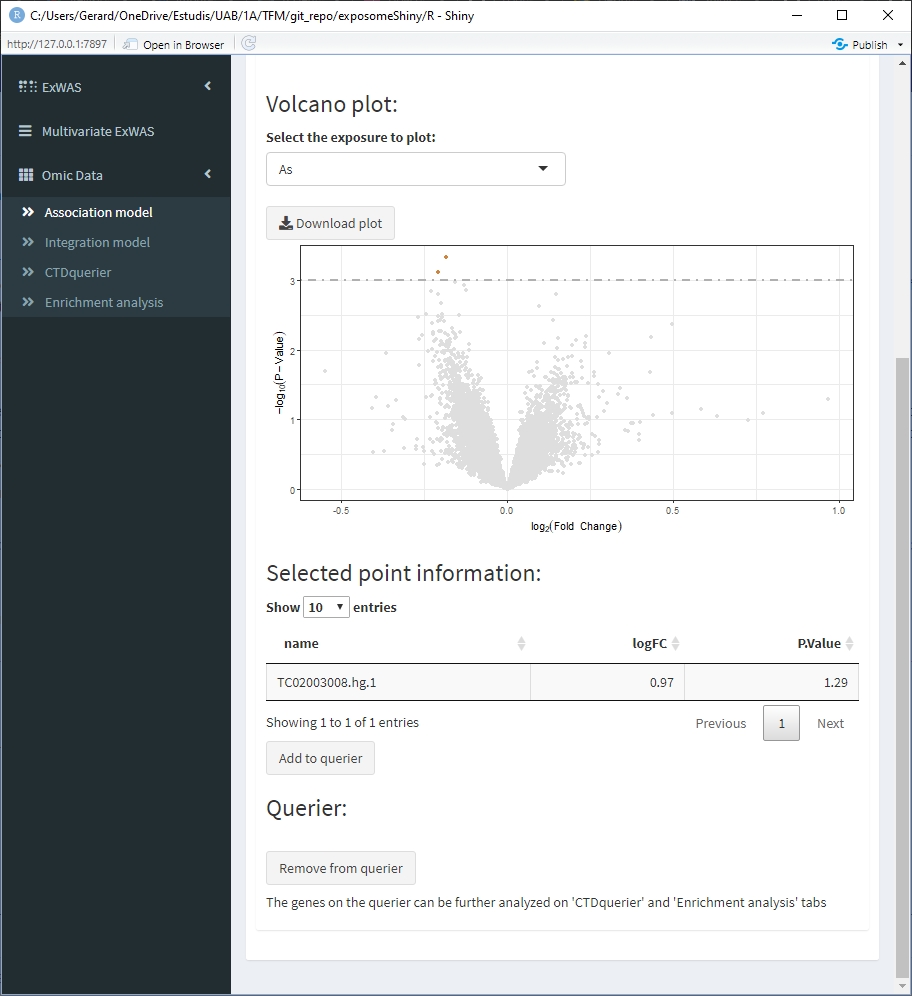
\includegraphics{images/analysis10_2.png}

If by mistake some gene (or genes) were introduced to the querier, select them by clicking on the table row and click ``Remove from querier''. Click on ``Query selected genes on the CTD gene database'' to perform the query of all the symbols of the querier list.

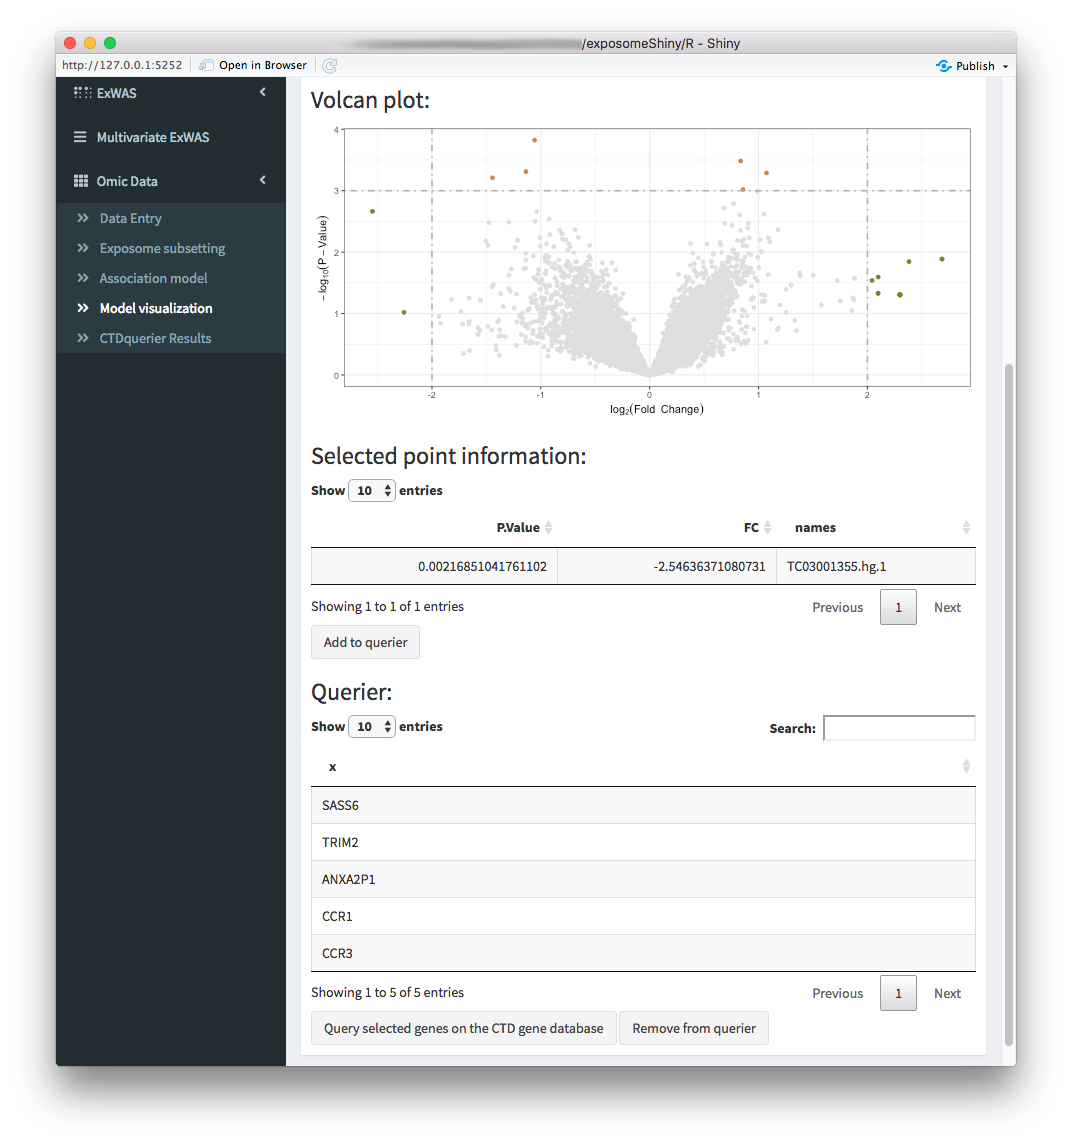
\includegraphics{images/analysis10_3.png}

To visualize the results of the query, go to the ``CTDquerier results'' subtab. There are six tabs showing different results interpretations. First there's the ``Lost \& found'' tab which a plot to see the amount of genes found on the CTD database and the ones that were not found them, ther's also two lists stating the names of them.

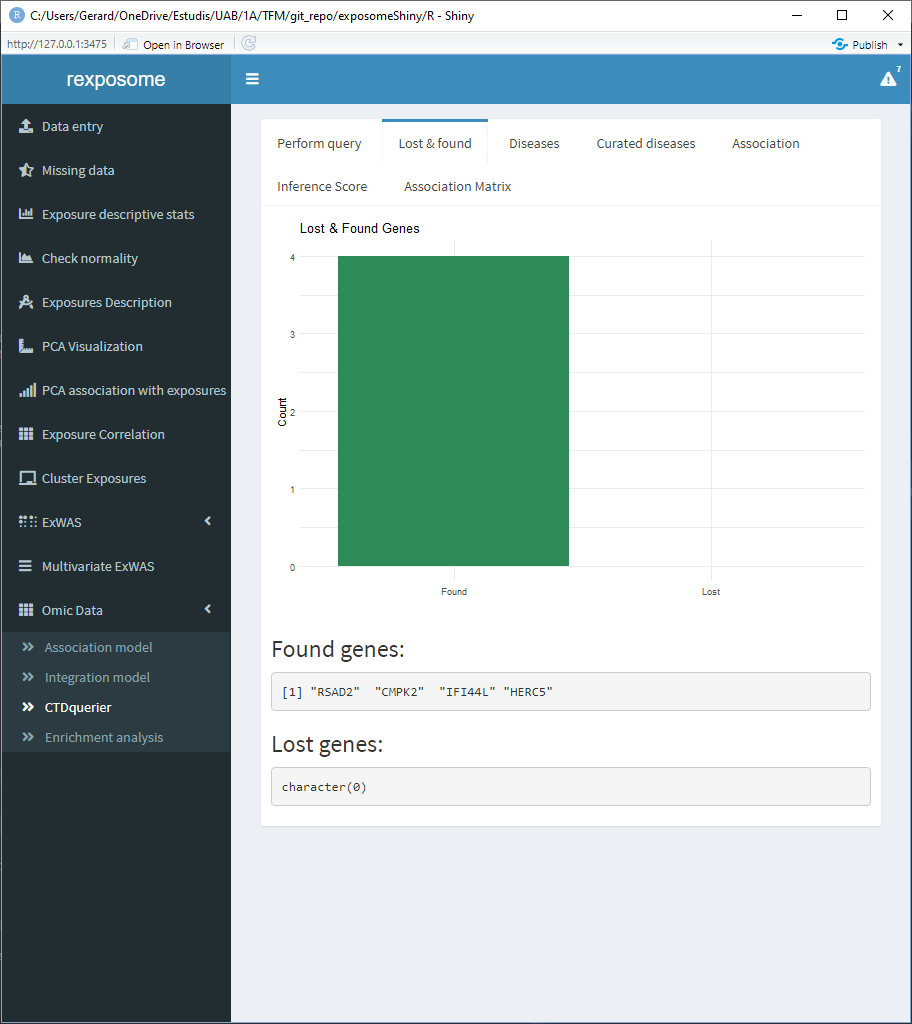
\includegraphics{images/analysis10_4.png}

The diseases tab shows a table of all the associated diseases found on the CTD database.

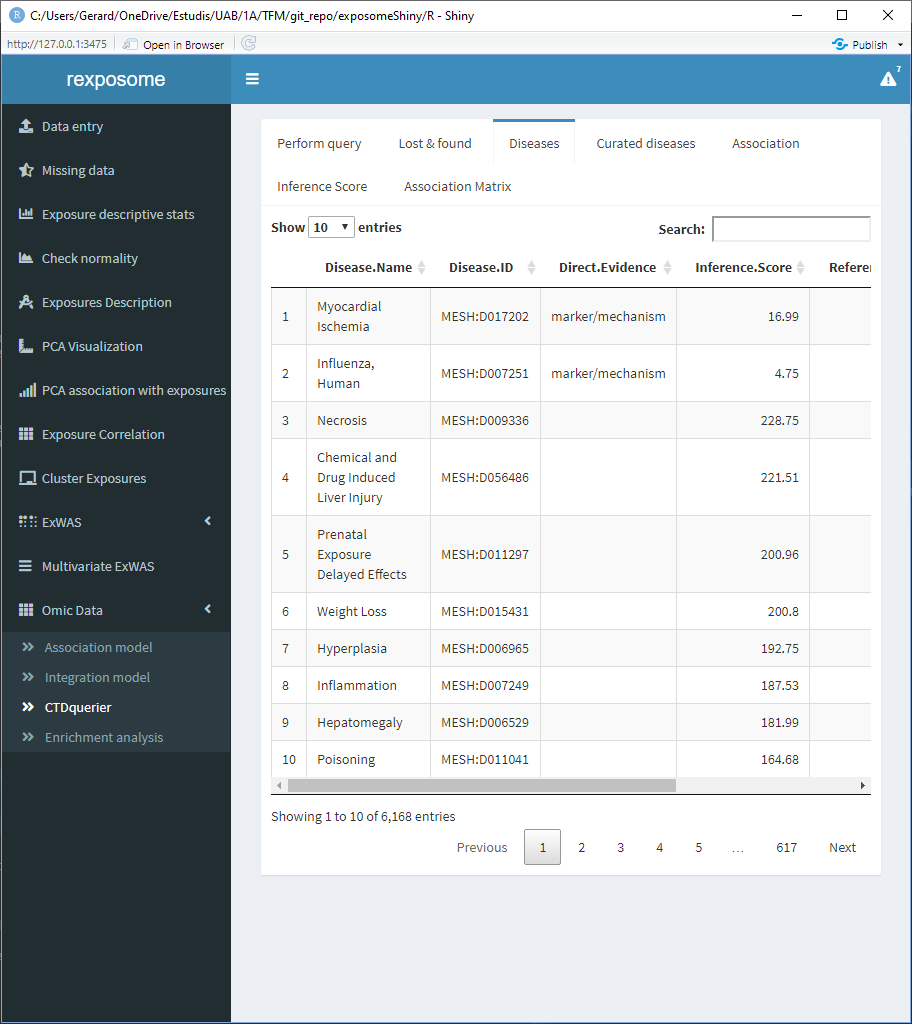
\includegraphics{images/analysis10_5.png}

The curated diseases tab shows the table of associated diseases but only shows the ones with direct evidence.

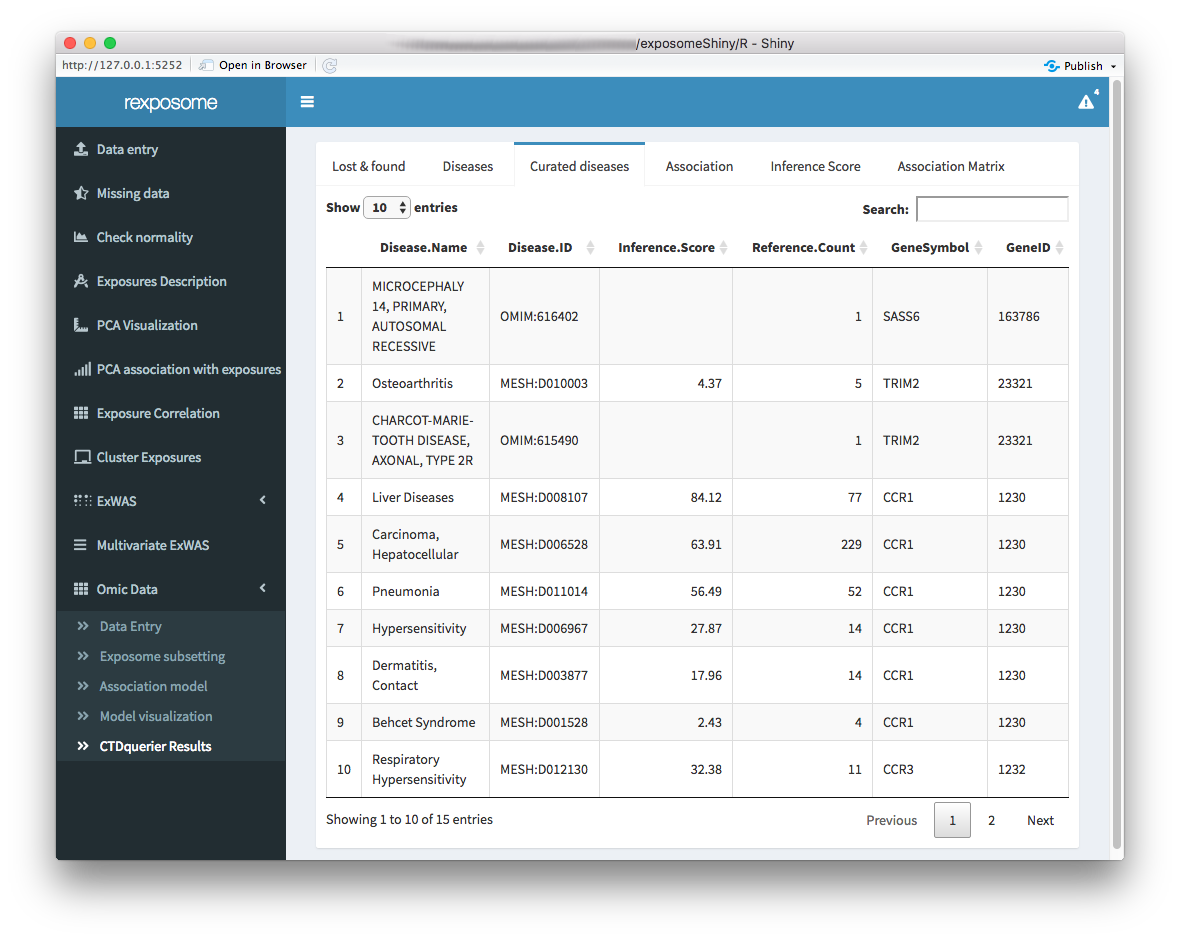
\includegraphics{images/analysis10_6.png}

The association tab shows information about all the direct evidence associated diseases. Select the disease of interest to see the score and reference count of it.

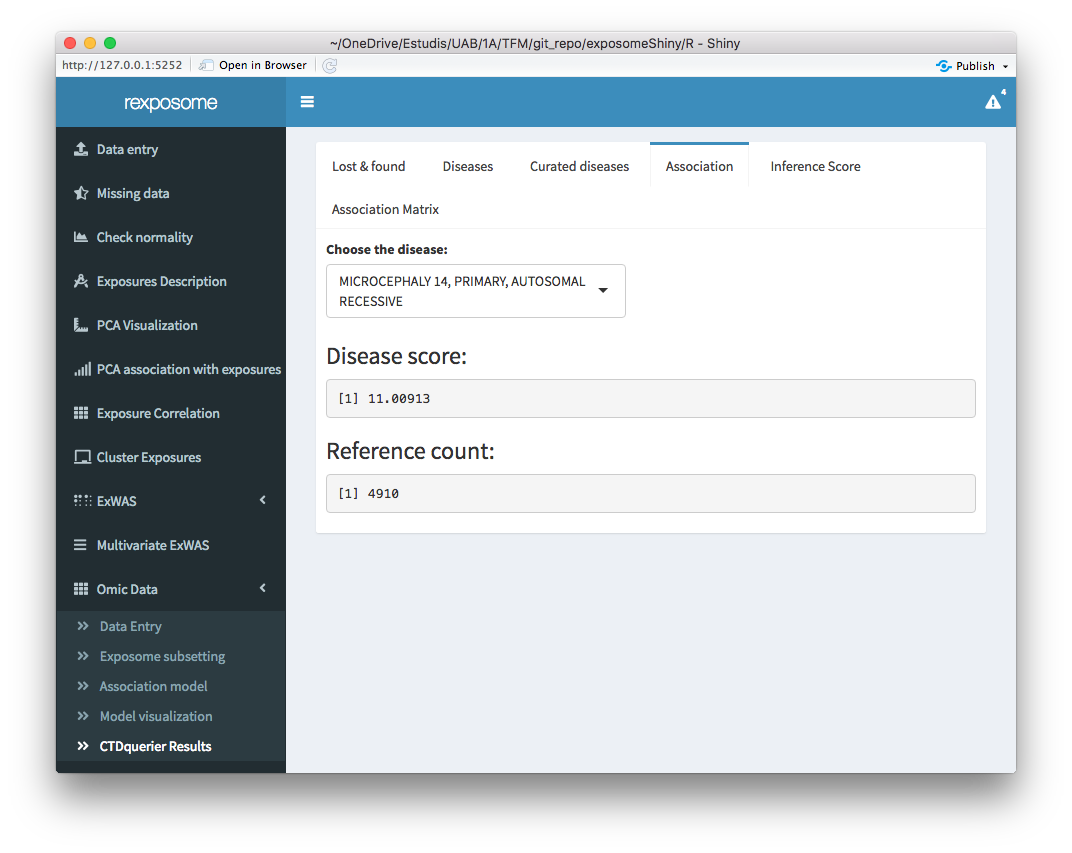
\includegraphics{images/analysis10_7.png}

The inference score tab shows the inference score for each gene for a selected disease, the filter parameters puts out the genes with an inference score lower than the selected filter.

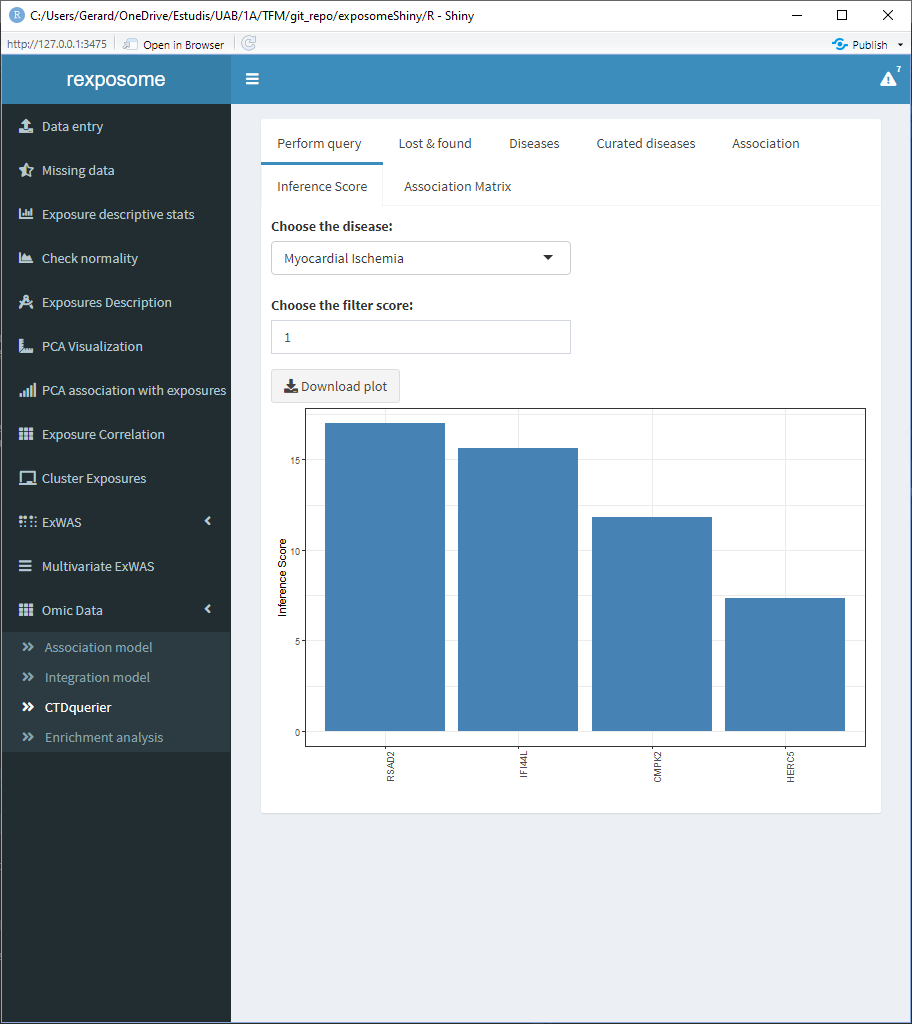
\includegraphics{images/analysis10_8.png}

The association matrix tab shows a matrix of genes vs.~chemicals with a heatmap representing the existing papers (references) providing evidence about the association between chemicals and genes.

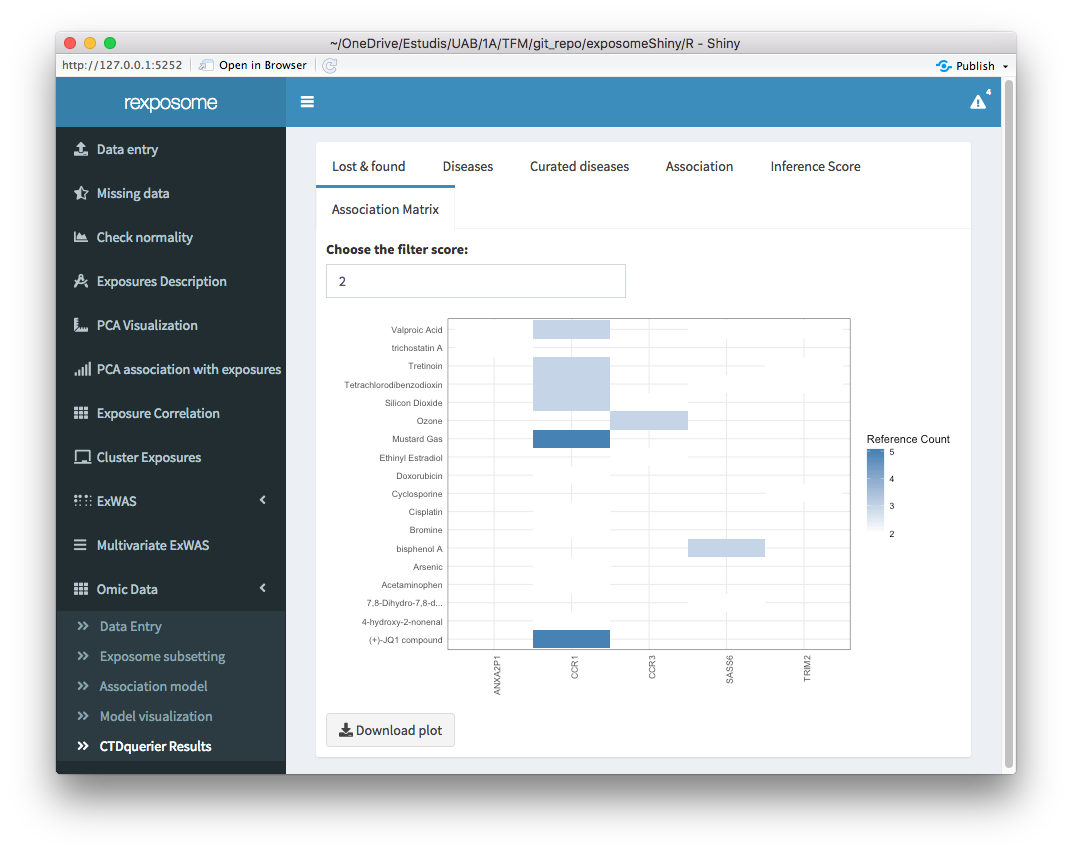
\includegraphics{images/analysis10_9.png}

\hypertarget{general-application-functionalities}{%
\chapter{General application functionalities}\label{general-application-functionalities}}

This whole Shiny application serves the purpose to perform a various number of exposome and omic analysis with an input set of data. To perform this analysis some operations can performed on the inputed dataset prior to the analysis and so in order to follow track of what exactly has been done or what is loaded on the current session, there's implemented some sort of state tracker inside the Shiny application. In order to access it, press the icon on the top right of the application

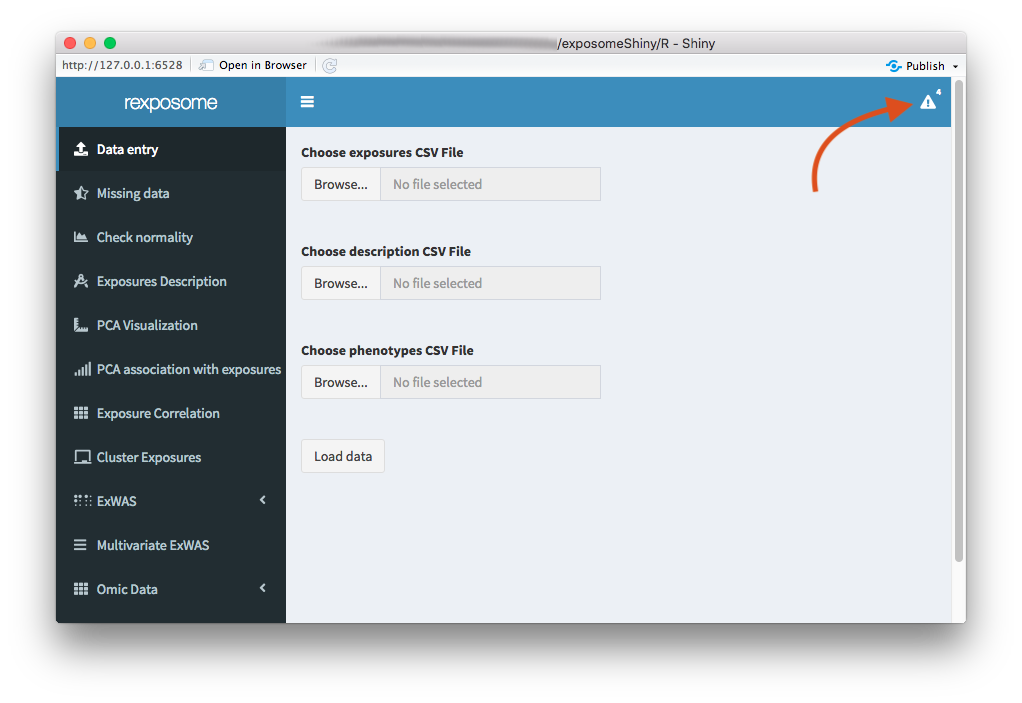
\includegraphics{images/general1.png}

When clicking it a dropdown menu appears, inside there are seven different notifications:

\begin{itemize}
\tightlist
\item
  Exposome dataset: Turns to 100\% when an exposome dataset is loaded in the environment. Here's a graphical example.

  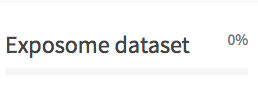
\includegraphics{images/general2.png}

  \includegraphics{images/general3.png}
\item
  LOD imputed: Turns to 100\% if the exposome dataset is LOD imputed.
\item
  Missing imputed: Turns to 100\% if the exposome dataset has the missings imputed.
\item
  Normality corrected: Turns to 100\% if the exposome dataset is normality corredted.
\item
  Omics dataset: Turns to 100\% when an omics dataset is loaded in the environment.
\item
  Subset: Turns to 100\% (and displays the subset family(ies)) when the exposome dataset is subseted.
\item
  Model: Turns to 100\% (and displays the association variable(s)) when a model is performed for an omics association analysis. Here's an example of a subset and model information.

  \includegraphics{images/general4.png}
\end{itemize}

  \bibliography{book.bib,packages.bib}

\end{document}
